\section{Αποτελέσματα}

\subsection{Προσομοιώσεις}
\label{ssec:simulations}
\paragraph{} Στην ενότητα αυτή παρουσιάζονται τα αποτελέσματα διαφόρων προσομοιώσεων. Τα
αποτελέσματα εξάγονται από το πρόγραμμα προσομοίωσης με τη μορφή αρχείων κειμένου
\eng{VTK}, τα οποία στη συνέχεια μπορούν να οπτικοποιηθούν και να διερευνηθούν διαδραστικά
μέσω διαφόρων ειδικών προγραμμάτων. Στην παρούσα εργασία, ως πρόγραμμα οπτικοποίησης
χρησιμοποιήθηκε το \eng{ParaView}, που αναπτύσσεται και διανέμεται ως ελεύθερο λογισμικό
από το \eng{Los Alamos National Laboratory}, το \eng{Sandia National Laboratory} και την
εταιρεία \eng{Kitware}. Το \eng{ParaView} τρέχει σε όλα τα ευρέως χρησιμοποιούμενα
λειτουργικά συστήματα (\eng{Unix/Linux, MS Windows, Mac OS X}), διαθέτει αρχιτεκτονική
\eng{client - server} για την οπτικοποίηση δεδομένων που βρίσκονται σε δίκτυο, υποστηρίζει
αρχιτεκτονικές κατανεμημένης επεξεργασίας ενώ δημιουργεί \eng{LOD} (\eng{Level of Detail})
οπτικοποιήσεις για την διατήρηση διαδραστικού αριθμού \eng{FPS} ακόμα και για μεγάλου
όγκου δεδομένα.

\begin{sidewaysfigure}
  \centering
  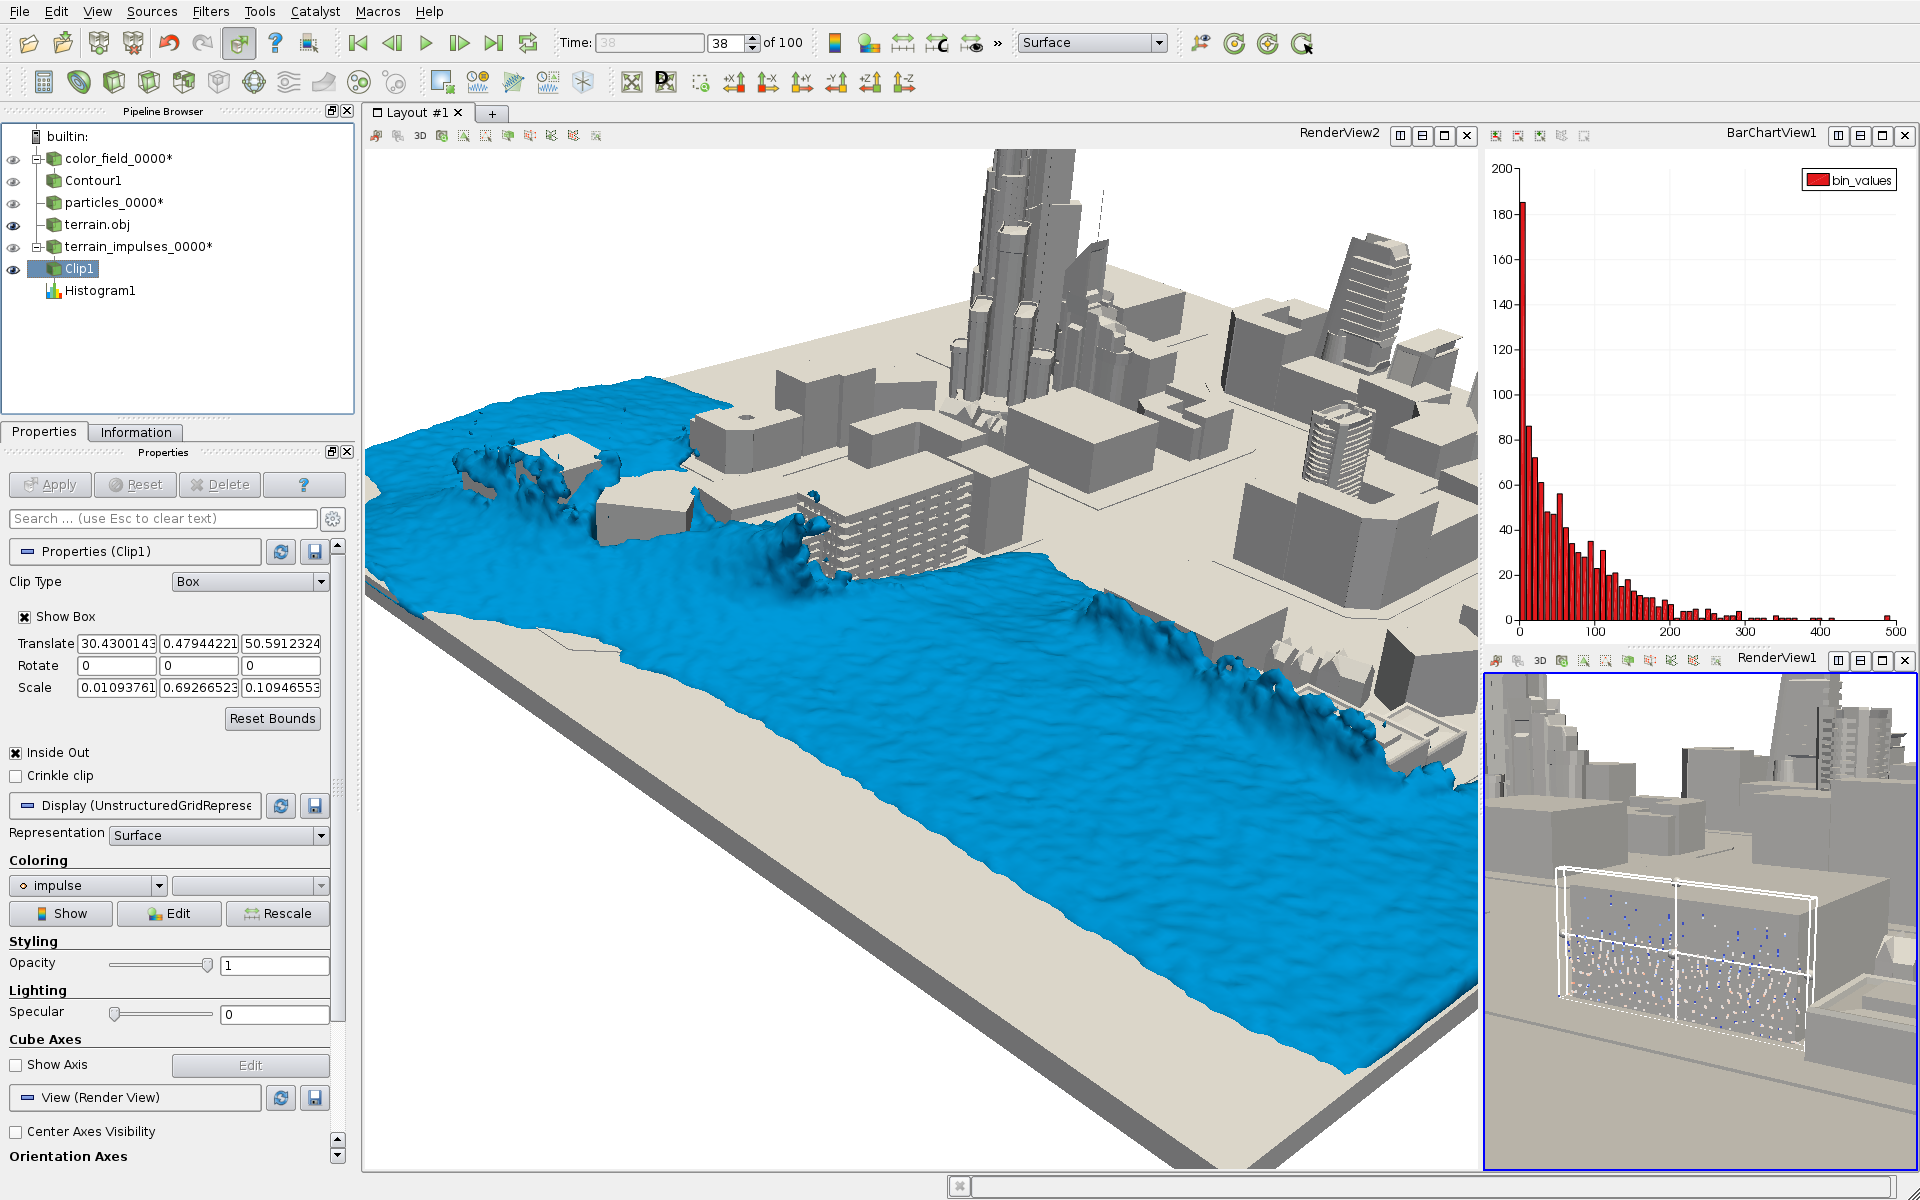
\includegraphics[width=\textwidth]{figures/paraview-interface.png}
  \caption[Οπτικοποίηση προσομοίωσης] {Οπτικοποίηση προσομοίωσης τσουνάμι \eng{85k}
    σωματιδίων στο \eng{ParaView}, στιγμιότυπο οθόνης. Αριστερά φαίνεται το ιεραρχικό
    δένδρο των δεδομένων που οπτικοποιούνται, στη μέση η ανακατασκευή της επιφάνειας του
    ρευστού σε συνδυασμό με το μοντέλο της ακτογραμμής, ενώ δεξιά οι ώσεις που ασκεί το
    ρευστό στο επιλεγμένο τμήμα του μοντέλου καθώς και γραφική απεικόνιση αυτών σε
    ιστόγραμμα.}
  \label{fig:paraview-interface}
\end{sidewaysfigure}

\paragraph{} Στην εικόνα \ref{fig:paraview-interface} φαίνεται σε στιγμιότυπο οθόνης το
περιβάλλον του \eng{ParaView} κατά την οπτικοποίηση μιας προσομοίωσης \eng{85k}
σωματιδίων. Στην αριστερή στήλη διακρίνεται το δένδρο με τις χρονοσειρές δεδομένων, στο
κορυφαίο επίπεδο του οποίου υπάρχουν το χρωματικό πεδίο (\eng{color\_field}), τα σωματίδια
της προσομοίωσης (\eng{particles}), οι ώσεις του ρευστού προς την ακτογραμμή
(\eng{terrain\_impulses}) και το μοντέλο της ακτογραμμής (\eng{terrain.obj}). Το ίδιο
σύνολο δεδομένων μπορεί να οπτικοποιηθεί ταυτόχρονα με πολλούς τρόπους, σε διάφορα
\eng{RenderViews}. Στο \eng{RenderView2} έχει επιλεγεί η απεικόνιση του μοντέλου της
ακτογραμμής σε γενική άποψη καθώς και της ισοεπιφάνειας του χρωματικού πεδίου, η οποία
δεδομένου ότι το χρωματικό πεδίο αντιπροσωπεύει την αδιάστατη πυκνότητα του ρευστού
αποτελεί μια αποδεκτή προσεγγιστική ανακατασκευή της επιφάνειάς του. Στο \eng{RenderView1}
έχει επιλεγεί η εστιασμένη απεικόνιση τμήματος της ακτογραμμής σε συνδυασμό με τις εντός
του κουτιού επιλογής (\eng{clip}) ώσεις προς αυτήν, οι οποίες είναι χρωματικά διαφορετικές
αναλόγως του μεγέθους τους και αναπαρίστανται σε ιστόγραμμα (\eng{BarChartView1}), όπου
είναι εύκολο να παρατηρηθεί η κατανομή της ορμής στα σωματίδια.

\begin{figure}[]
  \begin{subfigure}{.5\textwidth}
    \centering
    \includegraphics[width=\textwidth]{figures/press-0.png}
  \end{subfigure}
  \begin{subfigure}{.5\textwidth}
    \centering
    \includegraphics[width=\textwidth]{figures/press-1.png}
  \end{subfigure}
  \begin{subfigure}{.5\textwidth}
    \centering
    \includegraphics[width=\textwidth]{figures/press-2.png}
  \end{subfigure}
  \begin{subfigure}{.5\textwidth}
    \centering
    \includegraphics[width=\textwidth]{figures/press-3.png}
  \end{subfigure}
  \begin{subfigure}{.5\textwidth}
    \centering
    \includegraphics[width=\textwidth]{figures/press-4.png}
  \end{subfigure}
  \begin{subfigure}{.5\textwidth}
    \centering
    \includegraphics[width=\textwidth]{figures/press-5.png}
  \end{subfigure}
  \caption[Διάδοση δυνάμεων πίεσης]{Διαδοχικά στιγμιότυπα προσομοίωσης όπου αποτυπώνεται η
    διάδοση της ώσης του εδάφους στη υπερκείμενη στήλη νερού με τη μορφή δυνάμεων
    πίεσης. Τα σωματίδια της προσομοίωσης αναπαρίστανται με σημεία χρωματισμένα σύμφωνα με
    το μέτρο των δυνάμεων πίεσης που ασκούνται στο καθένα (θερμότητα χρώματος ανάλογη του
    μέτρου της δύναμης).}
  \label{fig:pressure-forces}
\end{figure}

\paragraph{} Όσον αφορά τις δυνάμεις που ασκούνται εντός του ρευστού, στις εικόνες
\ref{fig:pressure-forces} και \ref{fig:viscosity-forces} απεικονίζονται σε διαδοχικά
στιγμιότυπα τα σωματίδια της ίδιας προσομοίωσης, χρωματικά κωδικοποιημένα με βάση τις
δυνάμεις που ασκούνται σε αυτά λόγω πίεσης και ιξώδους αντίστοιχα. Το τσουνάμι
αναπαρίσταται σαν ένας όγκος νερού που εισβάλλει στην ακτογραμμή με μια σταθερή
ταχύτητα. Η προσέγγιση αυτή βρίσκεται αρκετά κοντά στην πραγματικότητα, δεδομένου οτι τα
τσουνάμι εκδηλώνονται ως μερικές επαναλαμβανόμενες, ορμητικές παλλίροιες της θάλασσας, με
μεγάλους όγκους νερού να ρέουν προς την ενδοχώρα. Στην εικόνα \ref{fig:pressure-forces}
παρατηρείται η διάδοση της ώσης του εδάφους στα αρχικά στάδια της προσομοίωσης μέσω
δυνάμεων πίεσης στη σχετικά άθικτη ακόμα υδάτινη στήλη (θερμότητα χρώματος ανάλογη του
μέτρου της δύναμης). Παρόμοια χρωματισμένες στην εικόνα \ref{fig:viscosity-forces}
διακρίνονται οι δυνάμεις ιξώδους, που οφείλονται στη διαφορά ταχύτητας μεταξύ γειτονικών
σωματιδίων και ως εκ τούτου είναι ισχυρές κατά την πρόσκρουση του ρευστού σε εμπόδια, όπου
τμήματά του αλλάζούν ταχύτητα σε σχέση με τα κοντινά τους. Στην εικόνα \ref{fig:samples}
τα σωματίδια κωδικοποιούνται χρωματικά σύμφωνα με το πλήθος γειτονικών σωματιδίων εντός
της ακτίνας εξομάλυνσης της προσομοίωσης. Όπως φαίνεται, λόγω της φύσης της προσομοίωσης
(ροή σε ανοιχτό χώρο με πολύπλοκα όρια) το ρευστό διαθέτει υψηλό λόγο επιφάνειας προς
όγκο, με αποτέλεσμα μεγάλο του μέρος να υποφέρει από υποδειγματοληψία. Για το λόγο αυτό
υιο\-θε\-τή\-θη\-καν (όπως αναλύθηκε και στην παράγραφο \ref{sssec:fluid-init})
γεωμετρικοί περιορισμοί μεταξύ των σωματιδίων για την αναπλήρωση της χαμένης πληροφορίας.

\begin{sidewaysfigure}[]
  \begin{subfigure}{.5\textwidth}
    \centering
    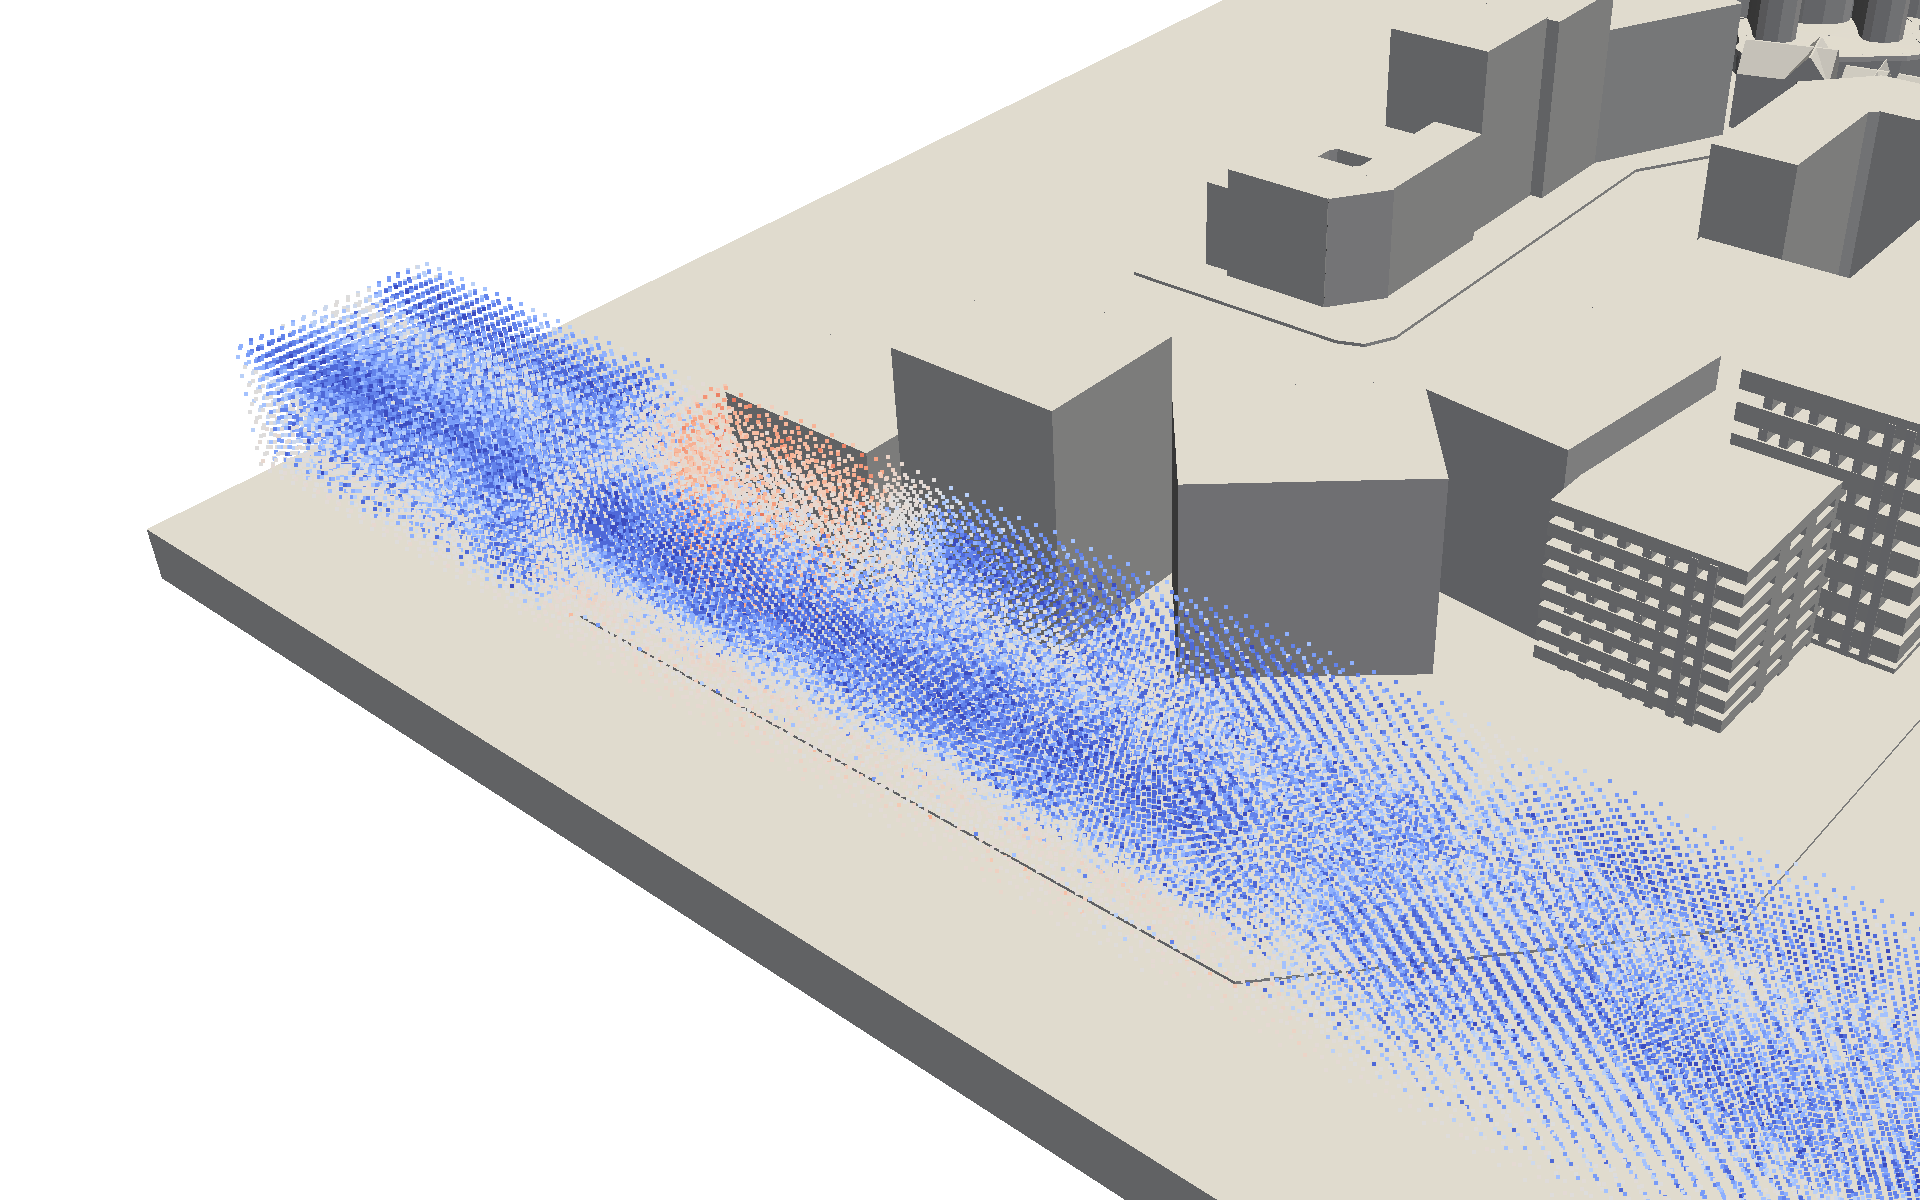
\includegraphics[width=\textwidth]{figures/visc-0.png}
  \end{subfigure}
  \begin{subfigure}{.5\textwidth}
    \centering
    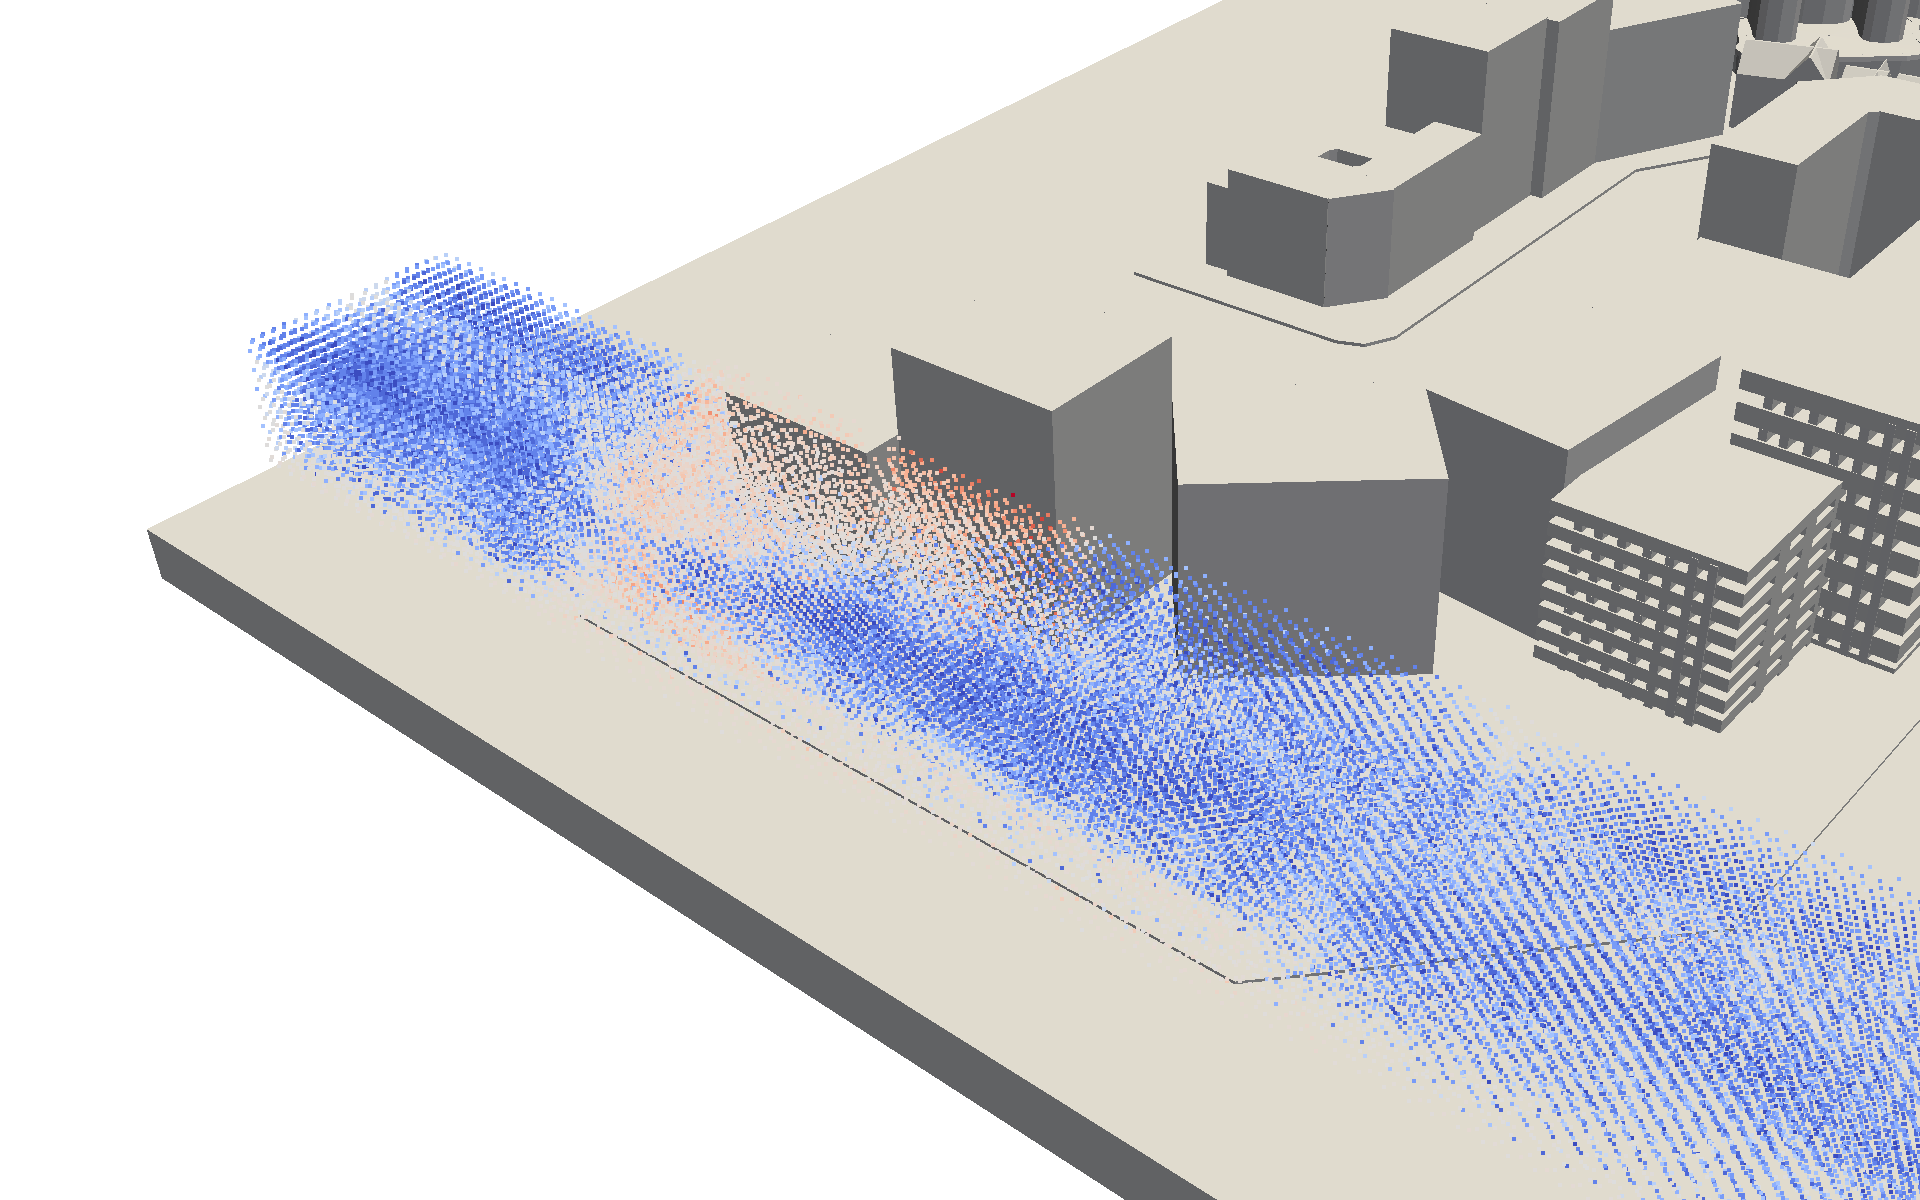
\includegraphics[width=\textwidth]{figures/visc-1.png}
  \end{subfigure}
  \begin{subfigure}{.5\textwidth}
    \centering
    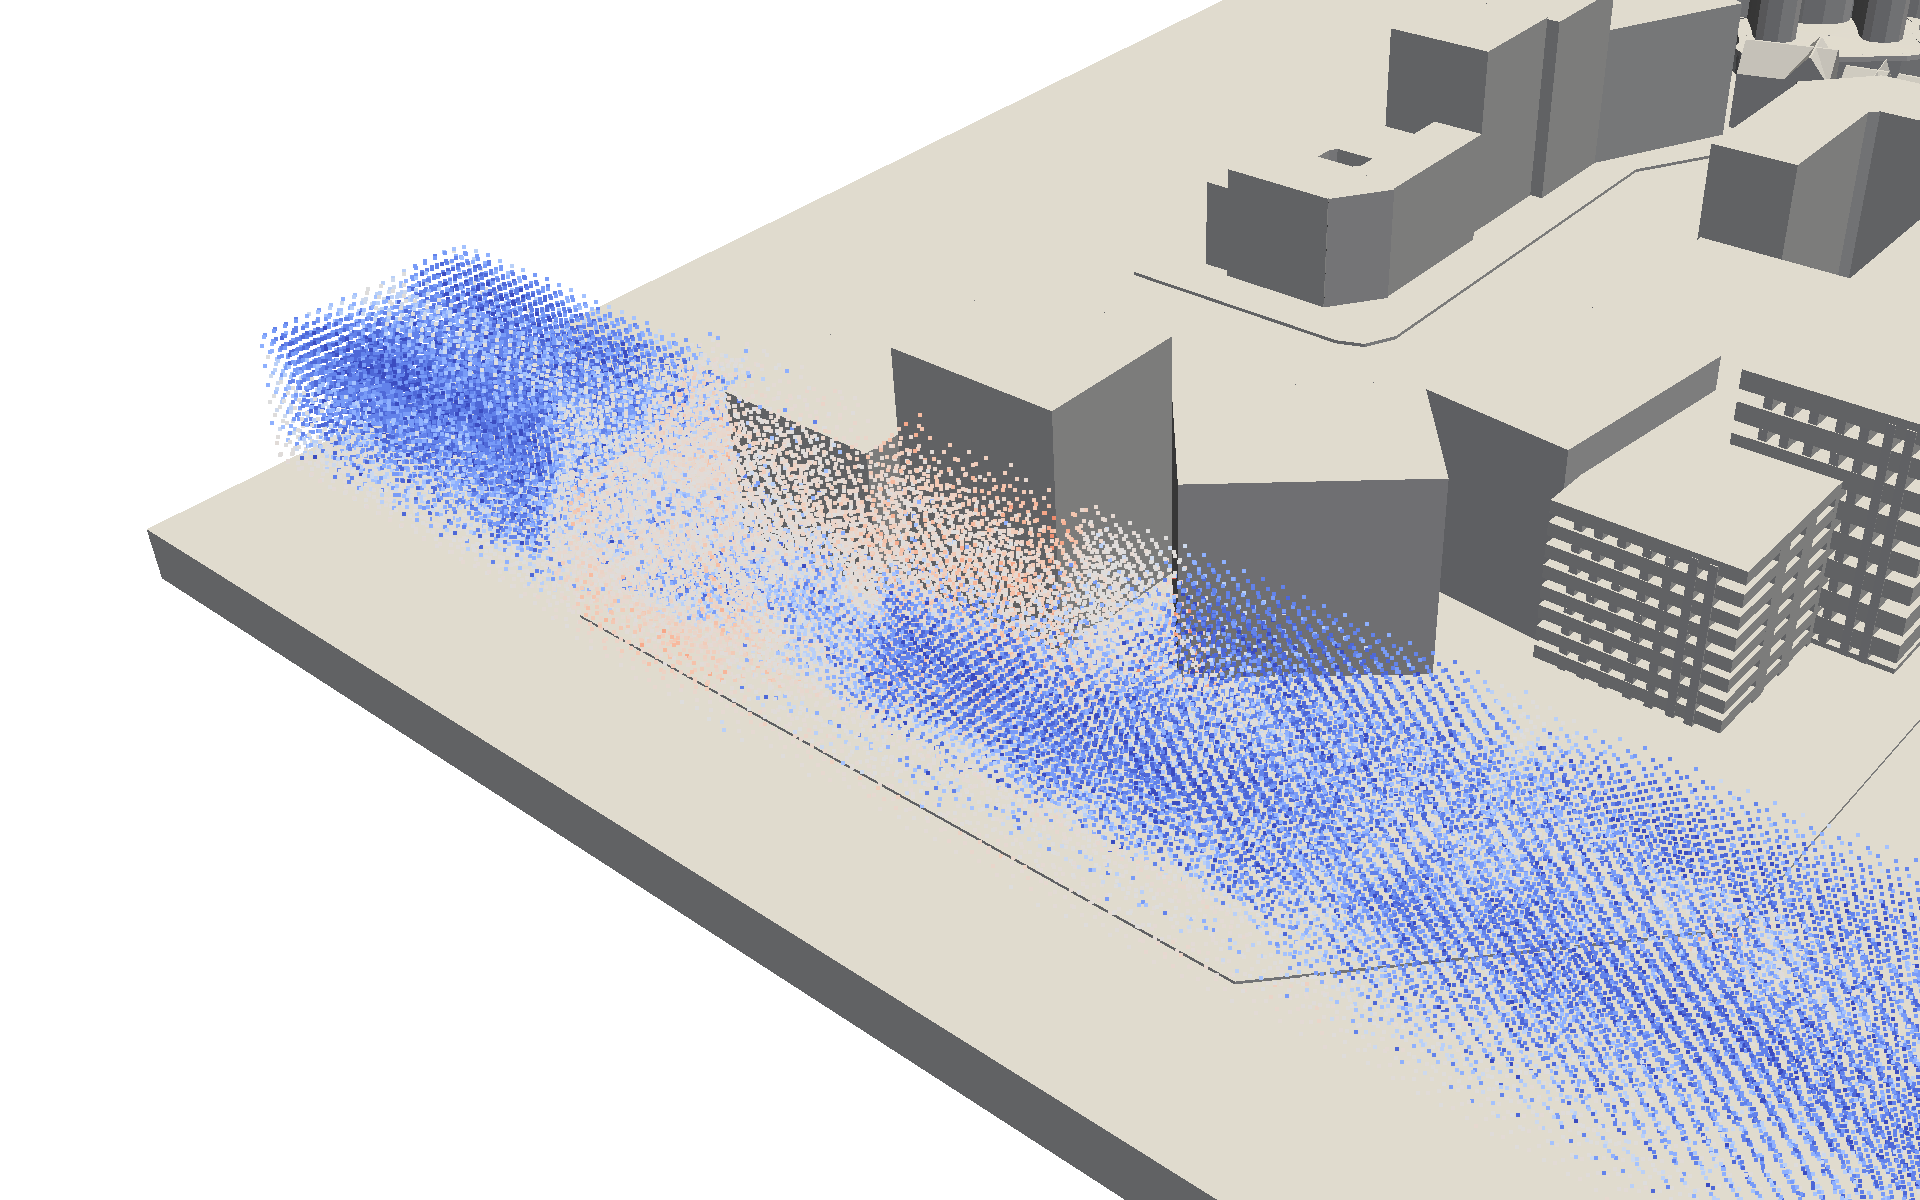
\includegraphics[width=\textwidth]{figures/visc-2.png}
  \end{subfigure}
  \begin{subfigure}{.5\textwidth}
    \centering
    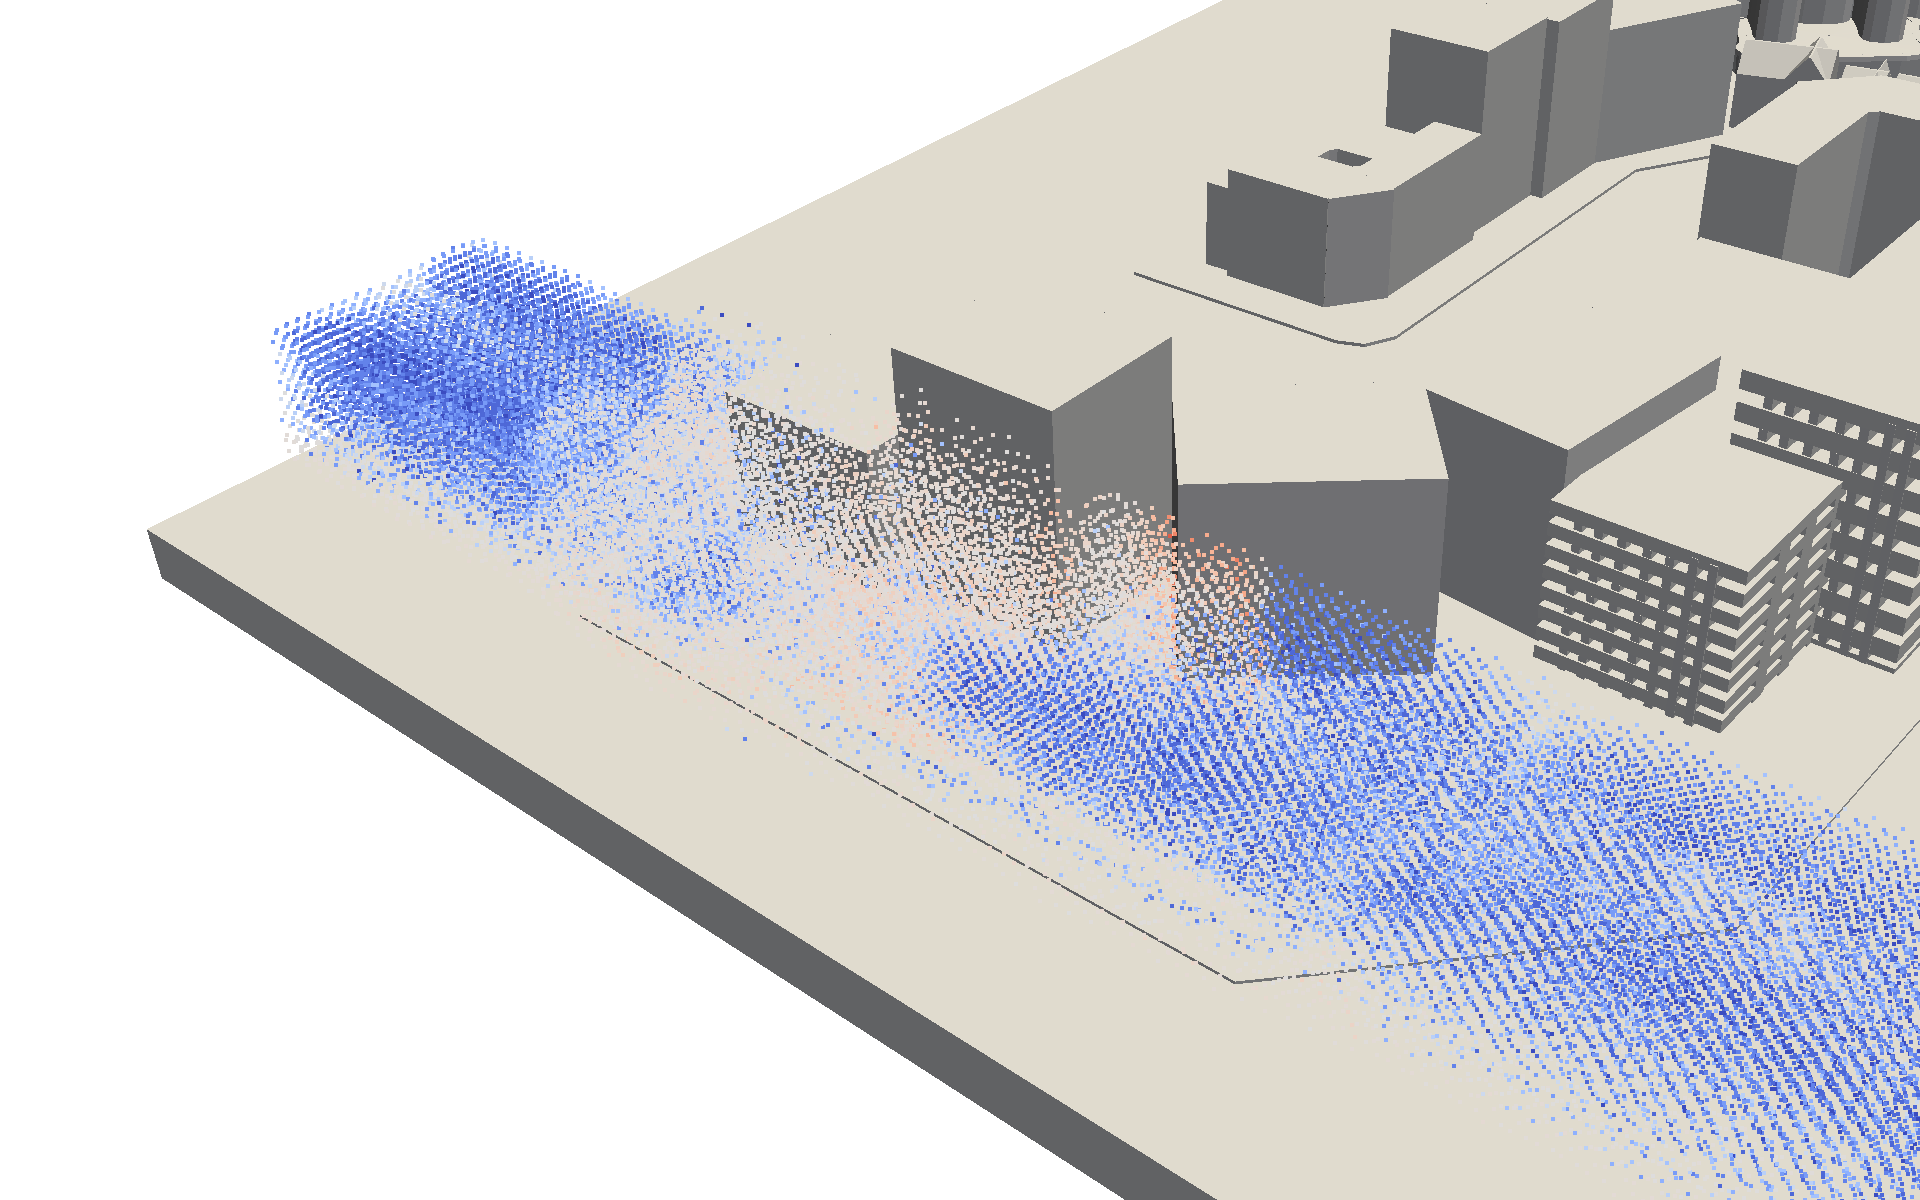
\includegraphics[width=\textwidth]{figures/visc-3.png}
  \end{subfigure}
  \caption[Δυνάμεις ιξώδους]{Διαδοχικά στιγμιότυπα προσομοίωσης όπου αποτυπώνεται
    χρωματικά στα σωματίδια το μέτρο της δύναμης που τους ασκείται λόγω ιξώδους του
    ρευστού. Η δύναμη του ιξώδους είναι ανάλογη της διαφοράς ταχύτητας μεταξύ γειτονικών
    σωματιδίων, και λόγω αυτού έχουν σημαντικό μέγεθος στις προσκρούσεις με εμπόδια,
    δεδομένης της απότομης αλλαγής ταχύτητας τμήματος του ρευστού (θερμότητα χρώματος
    ανάλογη του μέτρου της δύναμης).}
  \label{fig:viscosity-forces}
\end{sidewaysfigure}

\begin{sidewaysfigure}[]
  \centering
  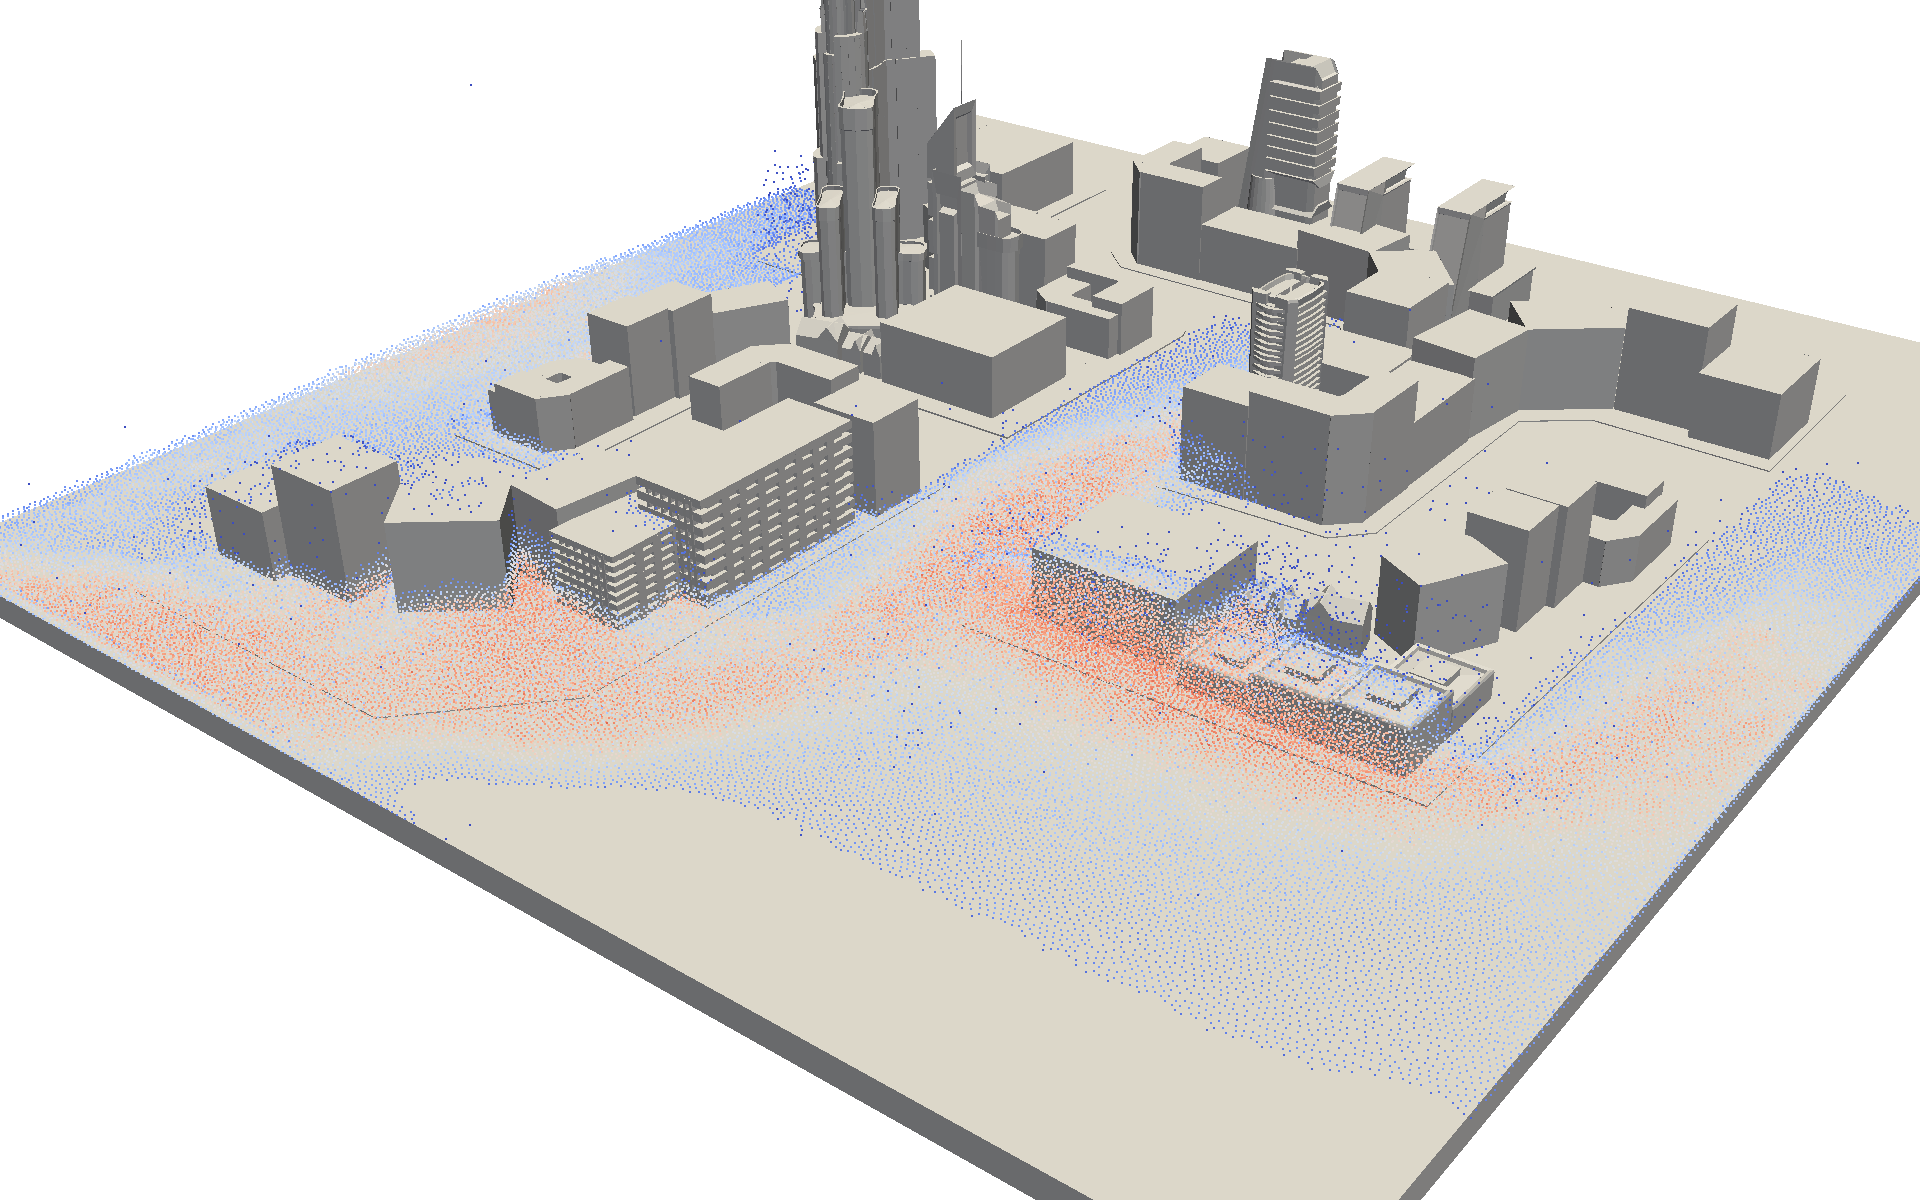
\includegraphics[width=\textwidth]{figures/samples.png}
  \caption[Απεικόνιση γειτονικών σωματιδίων] {Στιγμιότυπο προσομοίωσης όπου αναπαρίσταται
    χρωματικά ο αριθμός των δειγμάτων (γειτονικών σωματιδίων) που διατίθενται για την
    εκτίμηση των ιδιοτήτων του ρευστού (διακύμανση από σκούρο μπλε μέχρι έντονο κόκκινο, 0
    έως 52 δείγματα αντίστοιχα στην παρούσα περίπτωση). Λόγω της φύσης της προσομοίωσης
    (ροή σε ανοιχτό χώρο) είναι φανερή η έλλειψη ικανοποιητικού αριθμού δειγμάτων σε
    μεγάλο τμήμα του ρευστού, που οδήγησε και στην υιοθέτηση στοιχείων από \eng{PBD}
    (παράγραφος \ref{sssec:fluid-init}, \cite{Muller2007109, macklin2013position}).}
  \label{fig:samples}
\end{sidewaysfigure}

\begin{sidewaysfigure}[]
  \begin{subfigure}{.5\textwidth}
    \centering
    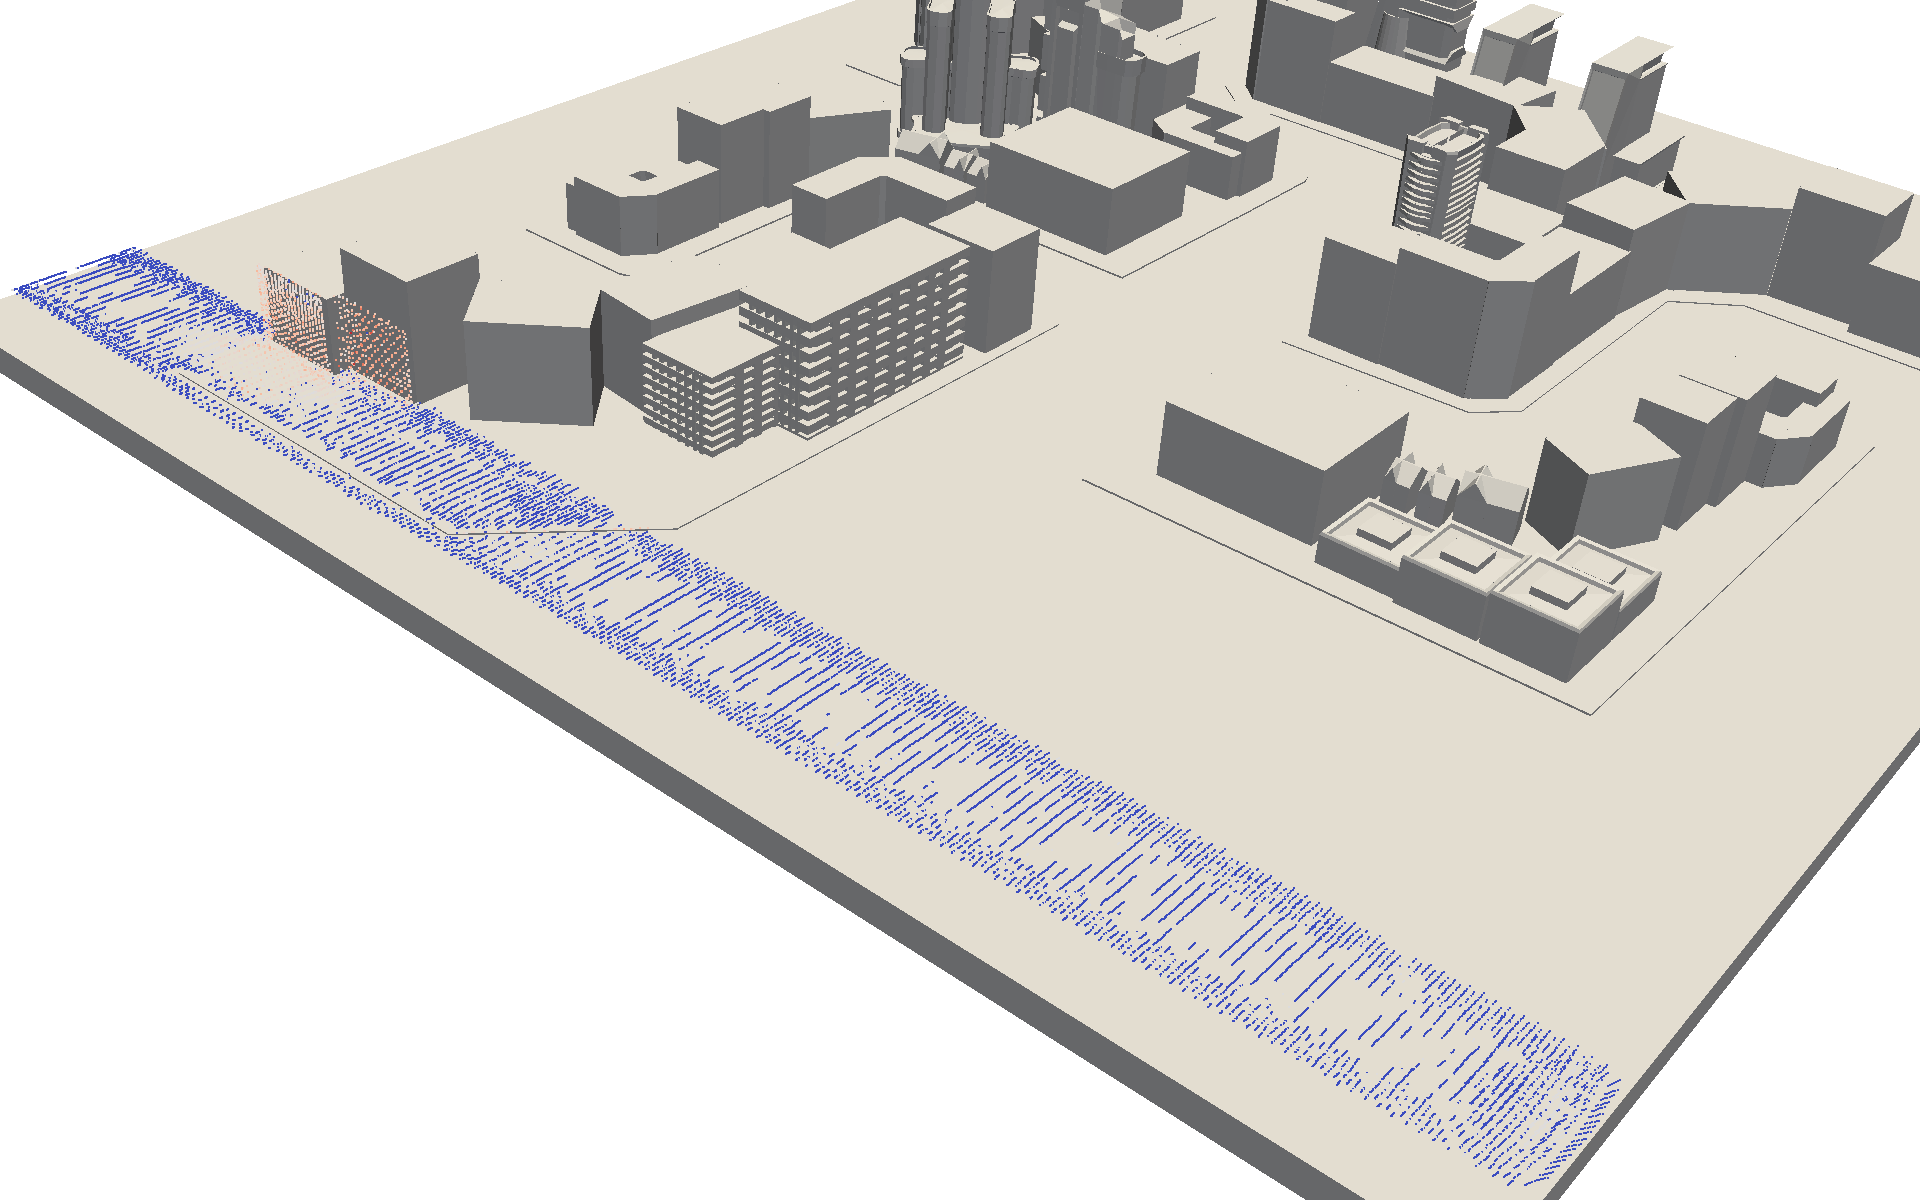
\includegraphics[width=\textwidth]{figures/impulses-0.png}
  \end{subfigure}
  \begin{subfigure}{.5\textwidth}
    \centering
    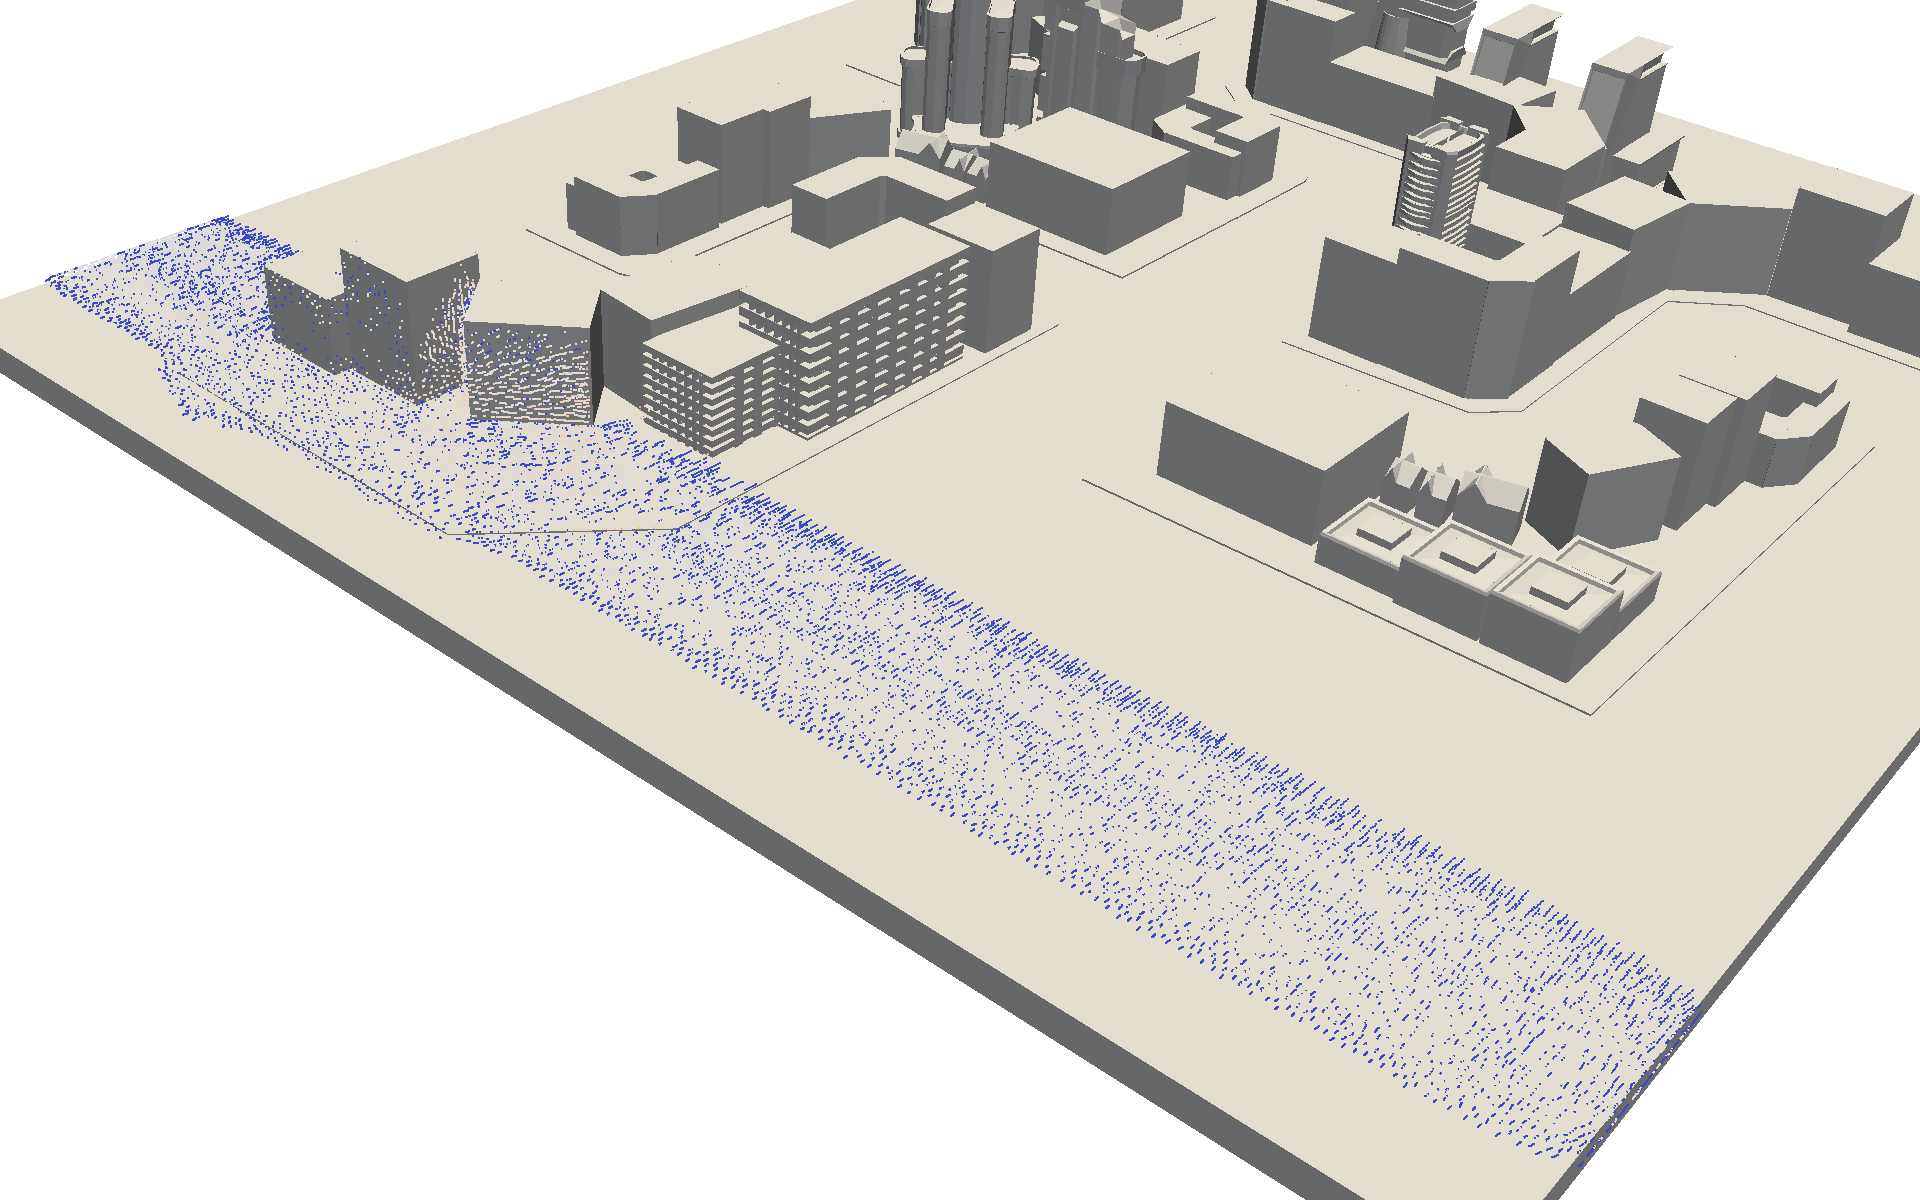
\includegraphics[width=\textwidth]{figures/impulses-1.png}
  \end{subfigure}
  \begin{subfigure}{.5\textwidth}
    \centering
    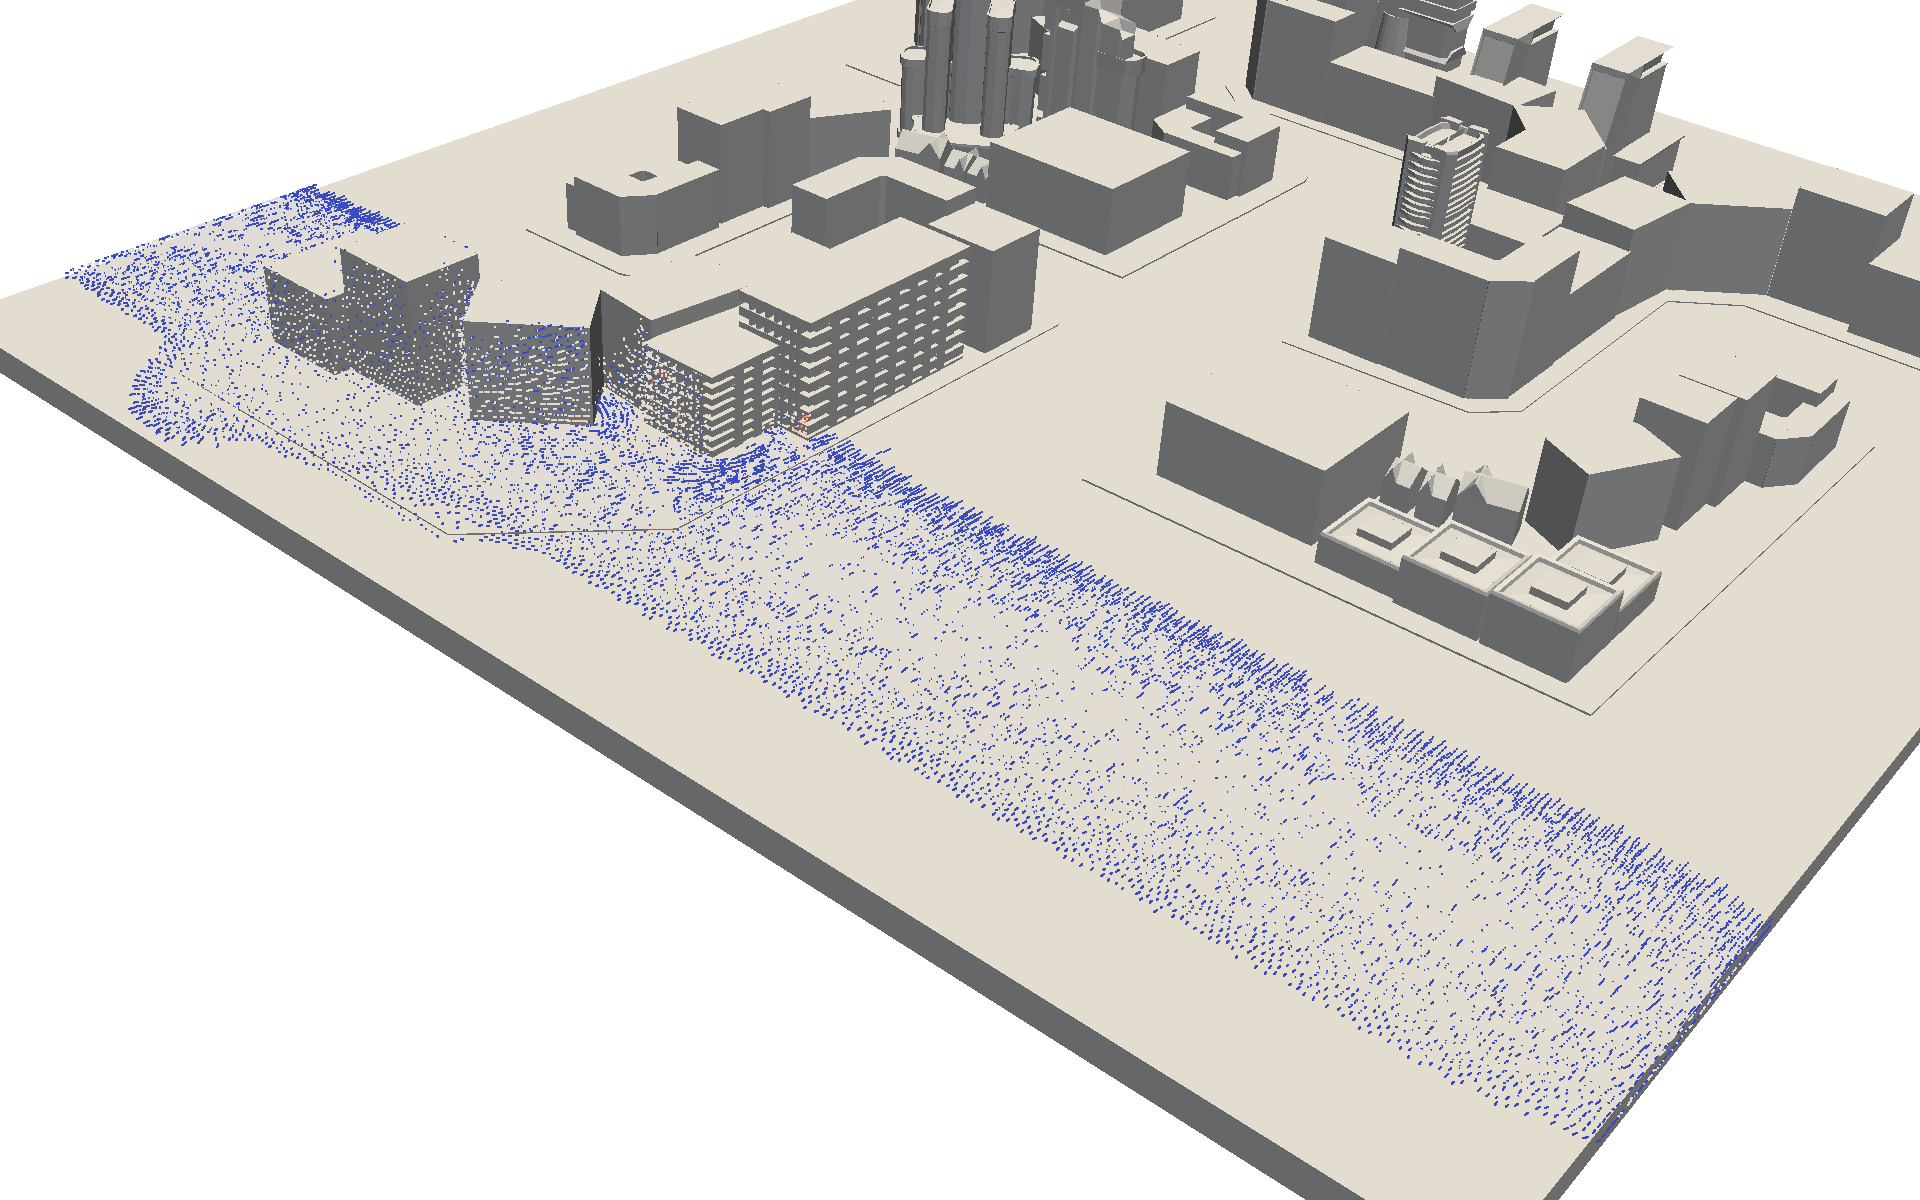
\includegraphics[width=\textwidth]{figures/impulses-2.png}
  \end{subfigure}
  \begin{subfigure}{.5\textwidth}
    \centering
    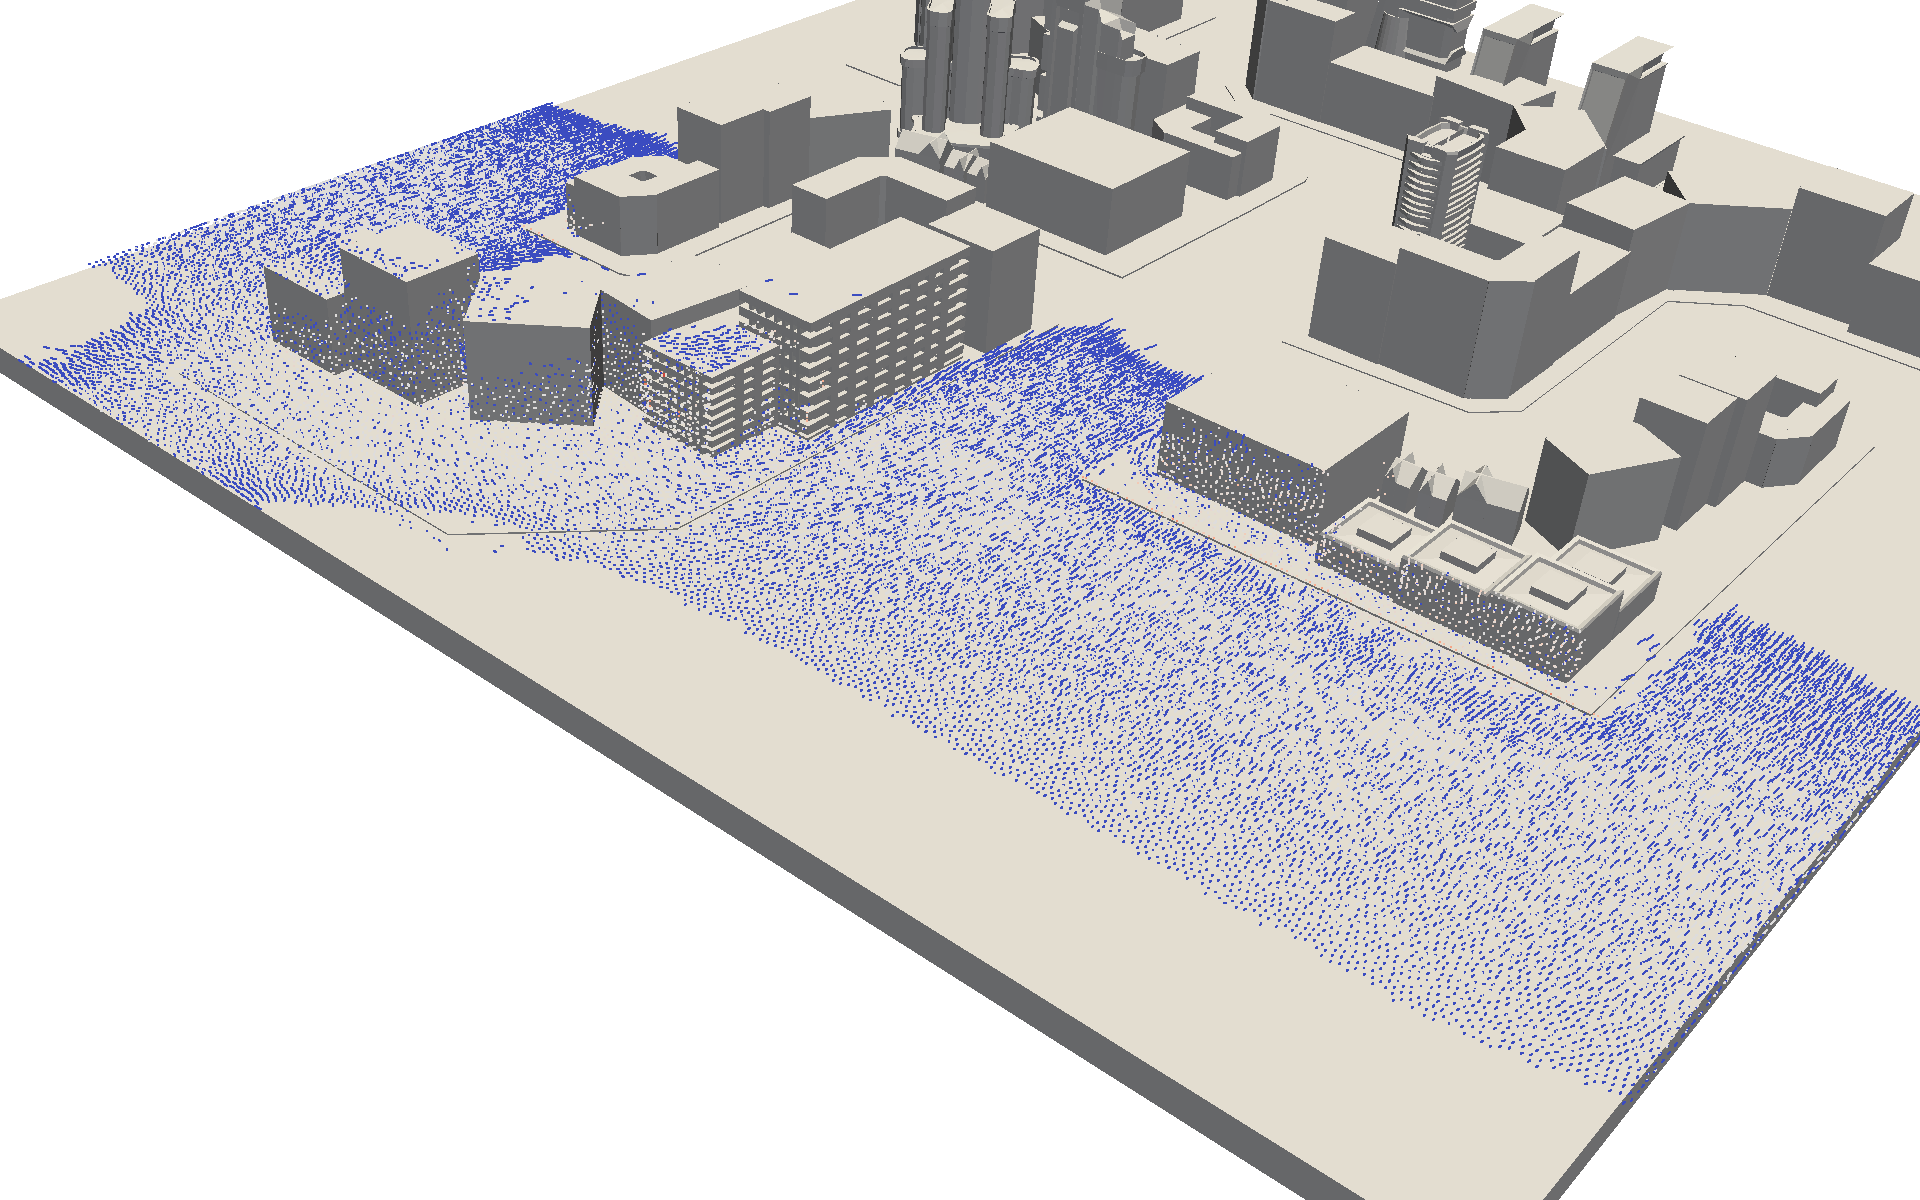
\includegraphics[width=\textwidth]{figures/impulses-3.png}
  \end{subfigure}
  \caption[Ώσεις στην ακτογραμμή]{Διάφορα στιγμιότυπα προσομοίωσης όπου αποτυπώνεται
    χρωματικά στην ακτογραμμή το μέτρο της ώσης που ασκείται από τα σωματίδια του ρευστού
    κατά την εξέλιξη του τσουνάμι (θερμότητα χρώματος ανάλογη του μέτρου της ώσης).}
  \label{fig:impulses}
\end{sidewaysfigure}

\begin{figure}[]
  \begin{subfigure}{.5\textwidth}
    \centering
    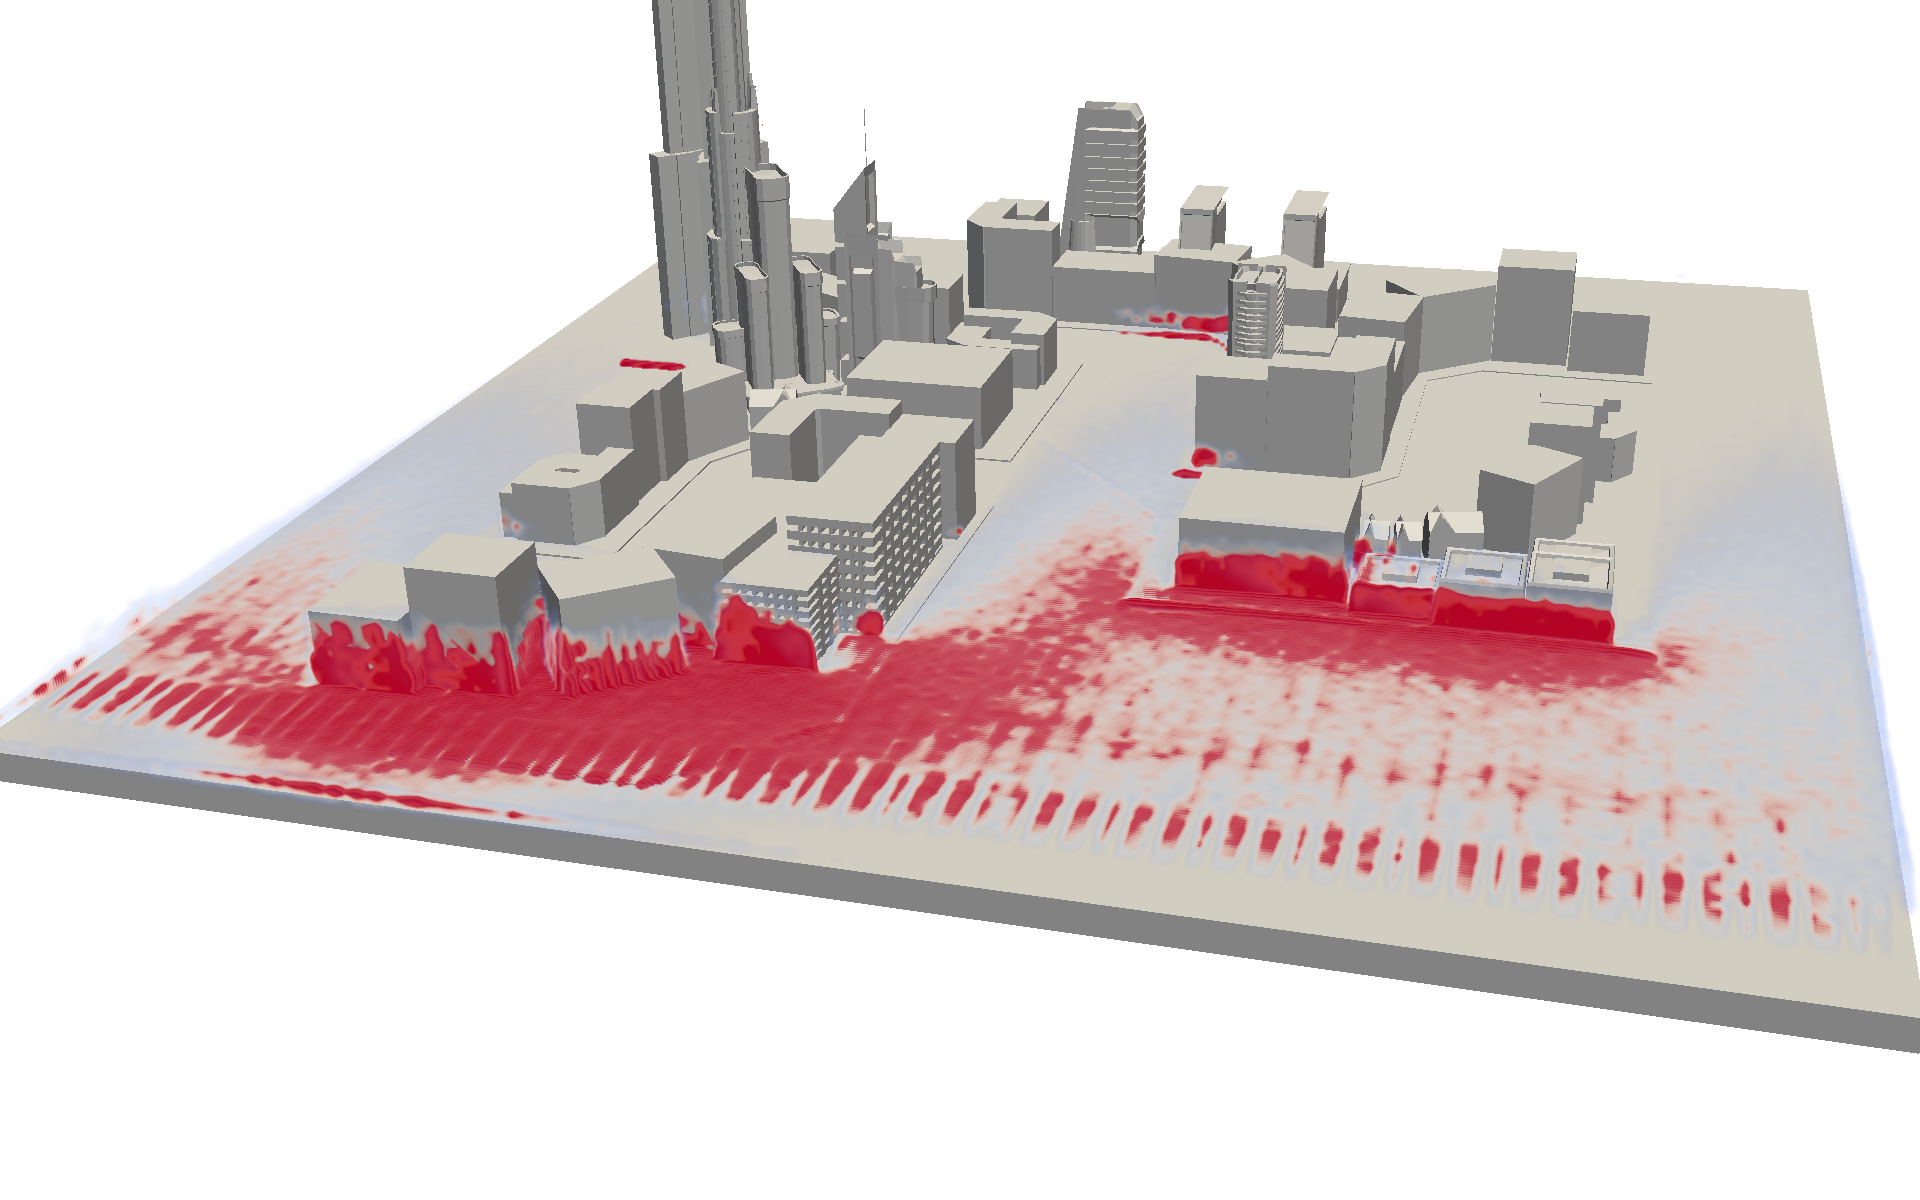
\includegraphics[width=\textwidth]{figures/impulse-heatmap-0.png}
  \end{subfigure}
  \begin{subfigure}{.5\textwidth}
    \centering
    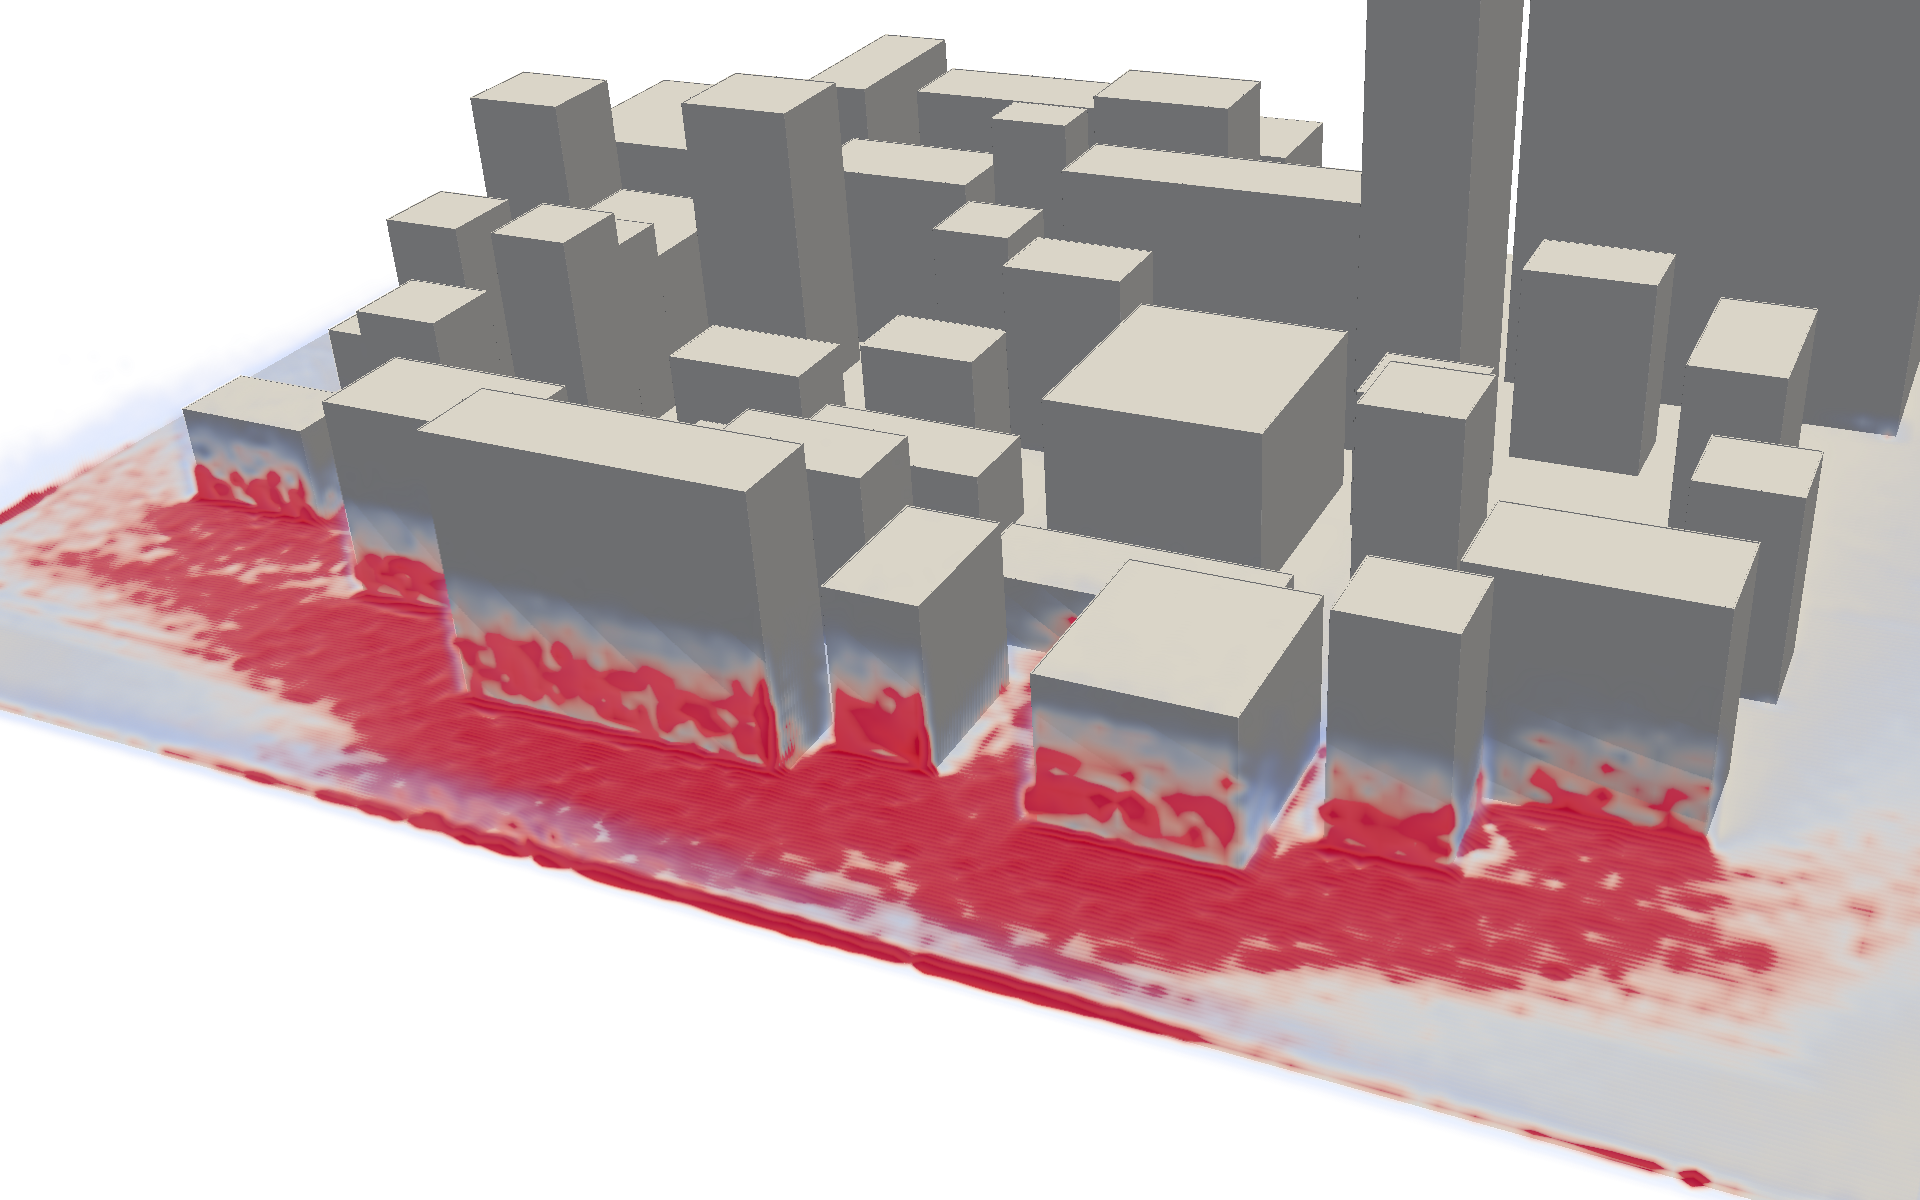
\includegraphics[width=\textwidth]{figures/impulse-heatmap-1.png}
  \end{subfigure}
  \begin{subfigure}{\textwidth}
    \centering
    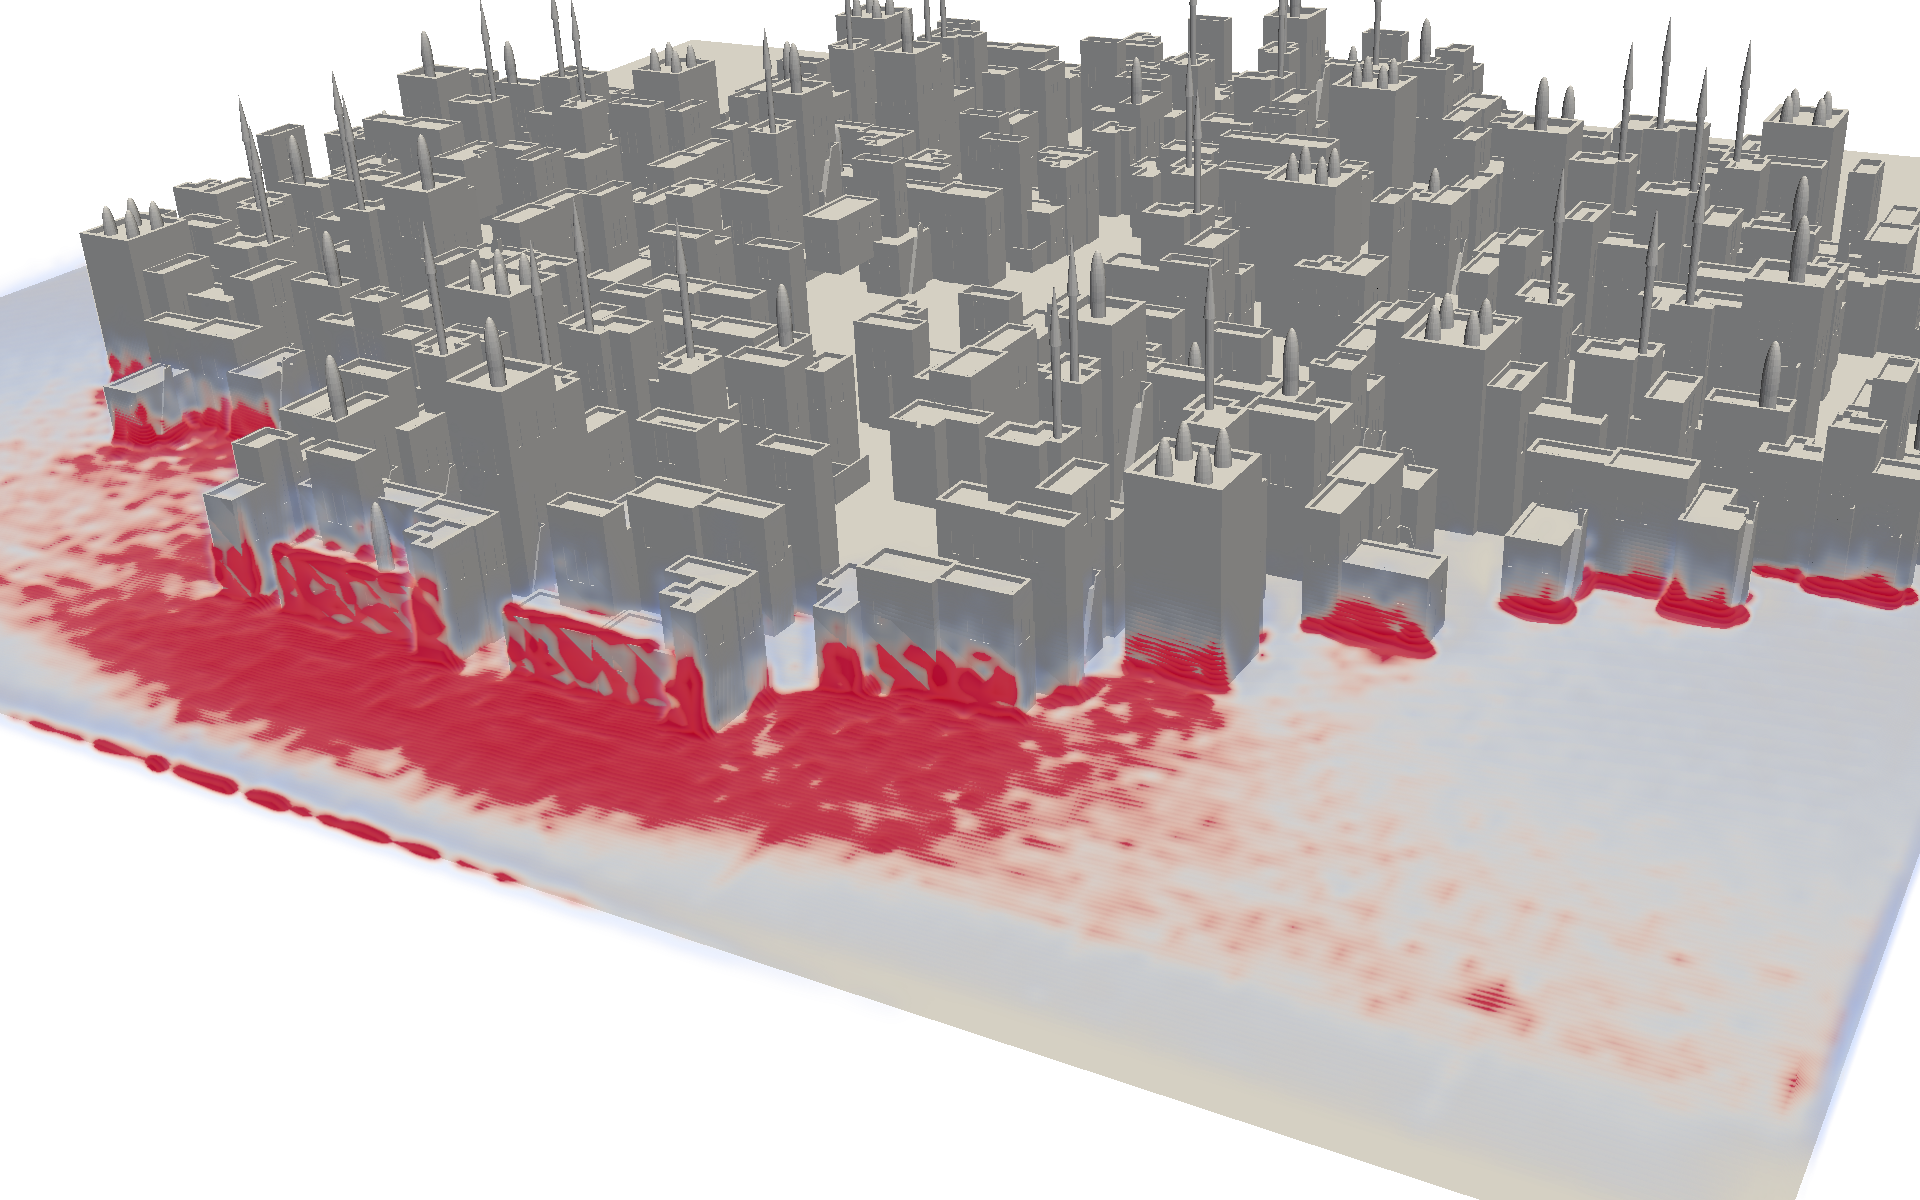
\includegraphics[width=\textwidth]{figures/impulse-heatmap-2.png}
  \end{subfigure}
  \caption[\eng{Heatmap} ώσεων στην ακτογραμμή]{\eng{Heatmap} των ώσεων του ρευστού προς
    την ακτογραμμή καθ' όλη την εξέλιξη του κύματος, σε τρία διαφορετικά μοντέλα
    πόλης. Επιβεβαιώνεται οτι το μεγαλύτερο μέρος της ενέργειας του κύματος απορροφάται
    από από τα πρώτα εμπόδια που αυτό συναντά, φαινόμενο που έχει δειχθεί τόσο σε
    καταγραφές πραγματικών περιστατικών, όσο και στη βιβλιογραφία.}
  \label{fig:impulse-fields}
\end{figure}

\subsection{Συμπεράσματα}
\paragraph{} Όπως φαίνεται στην εικόνα \ref{fig:impulse-fields}, έγιναν διάφορες
προσομοιώσεις πρόσπτωσης τσουνάμι έναντι αρκετών μοντέλων πόλεων, από τις οποίες
απεικονίζεται το \eng{heatmap} των ώσεων που ασκεί το κύμα στην ακτογραμμή, υπολογιζόμενο
αθροιστικά από όλες τις καταγραφόμενες ώσεις (παράγραφος \ref{sssec:simulation}). Όπως
εύκολα μπορεί να παρατηρηθεί και από την εικόνα \ref{fig:seawall-comparison}, όπου
συγκρίνονται τα \eng{heatmap} ώσεων παρουσία και μη ενός κυματοθραύστη, το μεγαλύτερο
μέρος της ενέργειας του κύματος απορροφάται από το πρώτο εμπόδιο που αυτό συναντά. Η
παρατήρηση αυτή έρχεται σε πλήρη συμφωνία τόσο με την εμπειρία από πραγματικά περιστατικά,
όσο και από άλλες αναφορές στη βιβλιογραφία. Χαρακτηριστικό παράδειγμα από πρόσφατο
κρούσμα τσουνάμι αποτελεί το τσουνάμι στον Ινδικό Ωκεανό στις 26 Δεκεμβρίου 2004, όπου
περιοχές που προστατεύονταν κατά μήκος της ακτογραμμής από δάση ριζοφόρων δέντρων
(\eng{mangroves}) υπέστησαν πολύ μικρότερο συγκριτικά πλήγμα \cite{danielsen2005asian,
  kathiresan2005601}, ενώ ποσοτικές προβλέψεις που προέκυψαν από προσεγγιστικές θεωρητικές
αναλύσεις του φαινομένου αυτού συμφωνούν με μετρήσεις μεγεθών του κύματος, όπως του ύψους
του \cite{yanagisawa200927}. Το γεγονός αυτό έχει οδηγήσει στην κατασκευή τεράστιων
κυματοθραυστών σε περιοχές με υψηλό κίνδυνο πλήγματος από τσουνάμι. Παράδειγμα επιτυχούς
αποτροπής σημαντικού πλήγματος αποτελεί η πόλη \eng{Pondicherry} στην Ινδία, η οποία
παρέμεινε σχεδόν άθικτη από το τεραστίου μεγέθους παραπάνω τσουνάμι εξαιτίας του τεράστιου
κυματοθραύστη που είχε κατασκευαστεί το 1735 από Γάλλους αποίκους και συνέχισε έκτοτε να
συντηρείται. Ωστόσο οι κυματοθραύστες δεν είναι πάντα αποτελεσματικοί. Η καταστροφή στο
πυρηνικό εργοστάσιο \eng{Fukushima Daiichi} το 2011 προκλήθηκε από το σεισμό και το
ακόλουθο τσουνάμι της περιοχής \eng{Tōhoku} στην Ιαπωνία, όταν τα κύματα ξεπέρασαν το ύψος
των κυματοθραυστών που προστάτευαν τις εγκαταστάσεις. Μεγάλη καταστροφή σημειώθηκε από το
ίδιο τσουνάμι και στην περιοχή \eng{Iwate}, παρά την εκτενή προστασία της από
κυματοθραύστες συνολικού μήκους 25 \eng{km}, καθώς τα κύματα ξεπέρασαν σε ύψος πάνω από
τους μισούς κυματοθραύστες. Οι κυματοθραύστες απορροφούν το μεγαλύτερο ποσοστό της
ενέργειας των κυμάτων, ωστόσο μεγάλο μέρος της ζημιάς που προκαλείται από τσουνάμι
οφείλεται στην πλημμύρα (\eng{flooding}) που προκαλείται σε εκτεταμένες περιοχές της
ακτογραμμής.

\begin{figure}[h!]
  \begin{subfigure}{\textwidth}
    \centering
    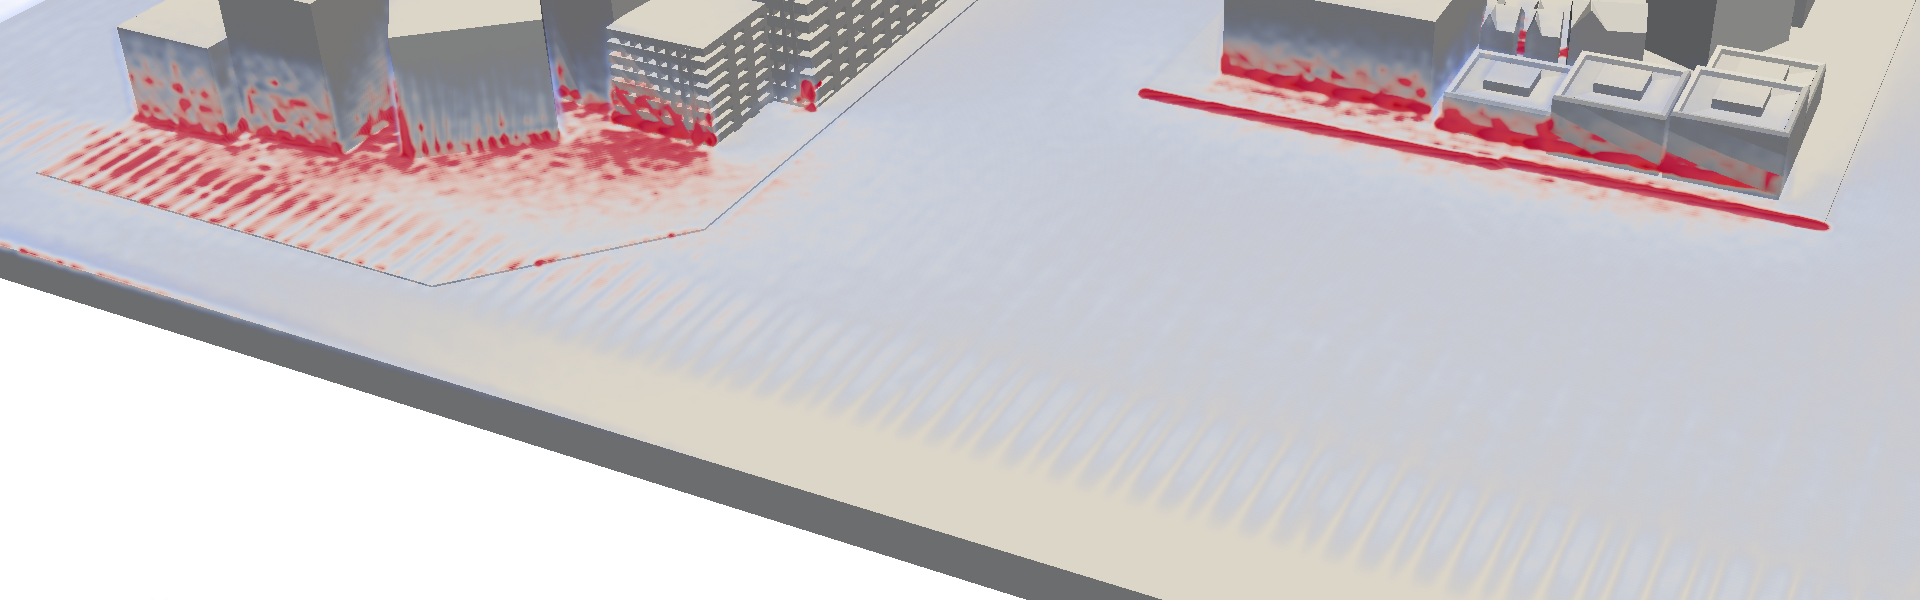
\includegraphics[width=\textwidth]{figures/if-city0-free.png}
  \end{subfigure}
  \begin{subfigure}{\textwidth}
    \centering
    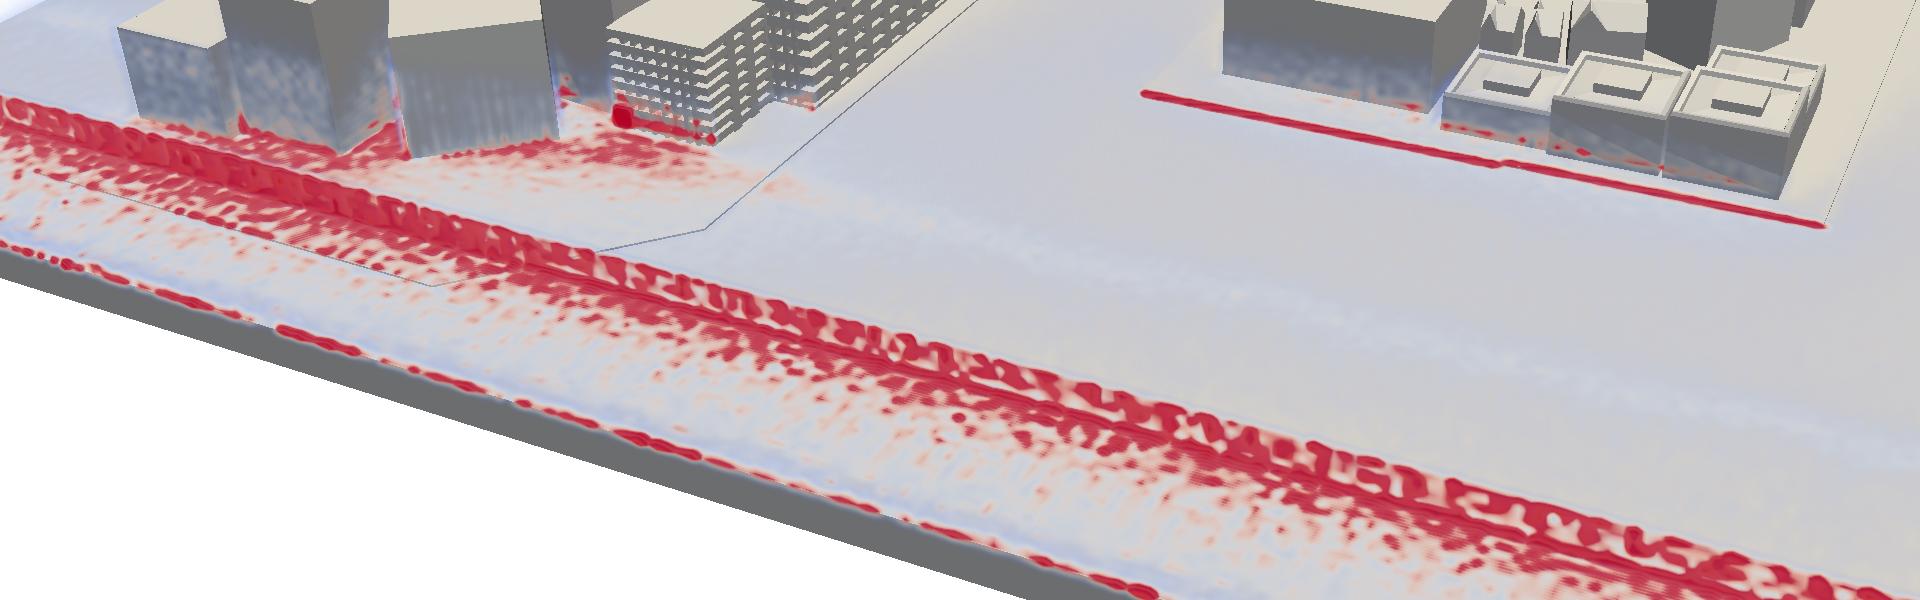
\includegraphics[width=\textwidth]{figures/if-city0-seawall.png}
  \end{subfigure}
  \caption[Συμβολή κυματοθραύστη στην αποτροπή ζημιάς]{Συγκριτική άποψη \eng{heatmap}
    ώσεων για το ίδιο μοντέλο πόλης και προσπίπτον κύμα, στην κάτω εικόνα προστατευόμενο
    από κυματοθραύστη. Είναι φανερή η μείωση των δυνάμεων από το κύμα στην ακτογραμμή στη
    δεύτερη περίπτωση.}
  \label{fig:seawall-comparison}
\end{figure}

\begin{figure}[h!]
  \centering
  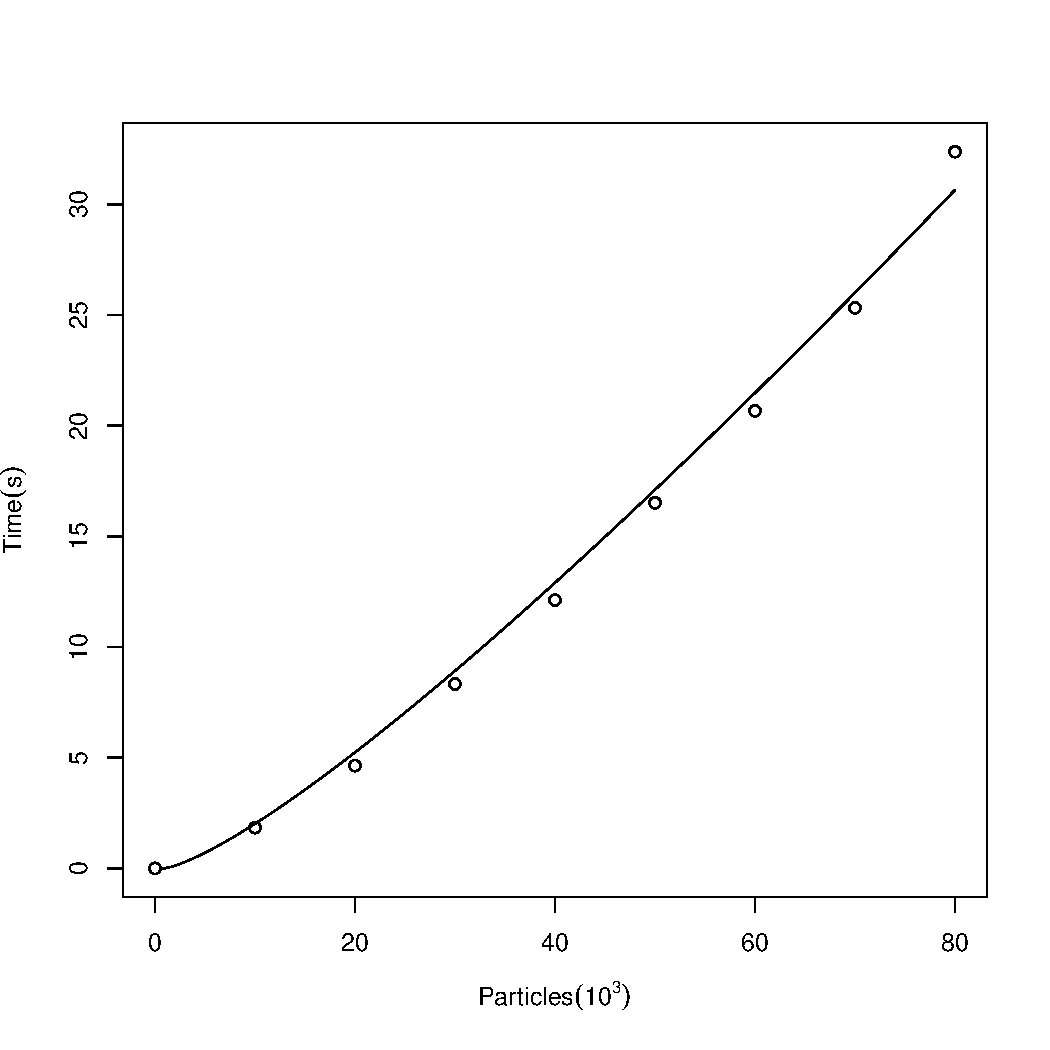
\includegraphics[width=\textwidth]{figures/performance.pdf}
  \caption[Απόδοση προγράμματος προσομοίωσης] {Γραφική παράσταση του μέσου χρόνου
    υπολογισμού ενός στιγμιοτύπου \eng{frame} συναρτήσει του αριθμού σωματιδίων,
    υπολογισμένου από τα 10 πρώτα στιγμιότυπα προσομοιώσεων με 10\eng{k} έως 80\eng{k}
    σωματίδια (η συνεχής γραμμή αναπαριστά $Ο(n log_2n)$ αύ\-ξη\-ση). Περίπου τα 75\% του
    χρόνου εκτέλεσης αντιστοιχούν σε σειριακό κώδικα διεργασιών της \eng{Bullet} και
    εξαγωγής δεδομένων, ενώ το 25\% σε παράλληλο κώδικα της μηχανής \eng{SPH}.}
  \label{fig:performance}
\end{figure}

\paragraph{} Στην εικόνα \ref{fig:performance} απεικονίζεται ο μέσος χρόνος υπολογισμού
ενός στιγμιοτύπου (\eng{frame}) συναρτήσει του αριθμού σωματιδίων, υπολογισμένου από τα 10
πρώτα στιγμιότυπα προσομοιώσεων με 10\eng{k} έως 80\eng{k} σωματίδια, σχέση η οποία
εκτιμάται να είναι τάξης $O(n log_2n)$ (συνεχής γραμμή). Λόγω των επιλεγμένων αρχικών
συνθηκών όπου τα σωματίδια βρίσκονται μόλις σε επαφή και στοιβαγμένα κατά το δυνατόν
συνεκτικότερα σε μικρό μέρος του τρισδιάστατου χώρου προσομοίωσης, τα πρώτα στιγμιότυπα
είναι κατά κανόνα αυτά με τον μεγαλύτερο υπολογιστικό φόρτο. Αν και οι συνθήκες αυτές δεν
επιτρέπουν την πλήρη συνεκτίμηση της επιτάχυνσης του προγράμματος από τη χρήση του \eng{LP
  grid} (δεδομένης της μη αξιοποίησης παρά μικρής έκτασης του πλέγματος), παρέχουν μια
αξιόπιστη εκτίμηση χειρότερης περίπτωσης (\eng{worst-case}) ανεξάρτητη από τη μορφολογία
της ακτογραμμής. Αξίζει στο σημείο αυτό να αναφερθεί, ότι από ανάλυση κατά την εκτέλεση
της εφαρμογής προέκυψε οτι περίπου το 75\% του χρόνου δαπανάται σε μονονηματικό
(\eng{single-threaded}) κώδικα, ο οποίος αποτελείται κυρίως από τις διεργασίες της
\eng{Bullet} και εισόδου-εξόδου (\eng{I/O}), ενώ μόνο το 25\% σε πολυνηματικό κώδικα ο
οποίος αφορά την ανίχνευση αλληλεπιδράσεων μεταξύ σωματιδίων και υπολογισμού χρωματικού
πεδίου. Μία άλλη παράμετρος που πρέπει να σημειωθεί είναι οτι πυκνότερη δειγματοληψία για
τον ίδιο όγκο νερού συνεπάγεται μικρότερη ακτίνα σωματιδίων και αυτό με τη σειρά του
μικρότερο εσωτερικό χρονικό βήμα (σύμφωνα με τις παραγράφους \ref{sssec:integration} και
\ref{sssec:fluid-init}), άρα περισσότερα εσωτερικά βήματα εντός ενός στιγμιοτύπου.

\paragraph{} Σε γενικές γραμμές η ποσοτική εκτίμηση της βελτίωσης στην ταχύτητα του
προγράμματος που επιτυγχάνεται με τη χρήση του \eng{LP grid} είναι δύσκολη, δεδομένου οτι
εξαρτάται από παραμέτρους της προσομοίωσης (αρχικές συνθήκες, δειγματοληψία, εσωτερική
αναπαράσταση σωματιδίων), μοτίβων πρόσβασης στα σωματίδια αλλά και του υλικού του
υπολογιστικού συστήματος (μεγέθος της κρυφής μνήμης). Τα αδιαμφισβήτητα πλεονεκτήματά του
περιλαμβάνουν:
\begin{itemize}
\item Συνεκτική αποθήκευση των σωματιδίων. Δεσμεύεται χώρος στη μνήμη ακριβώς ίσος με τον
  ελάχιστο δυνατό βάσει του μεγέθους της εσωτερικής αναπαράστασης των σωματιδίων.
\item Γρήγορη $Ο(1)$ πρόσβαση. Η ανάκτηση των σωματιδίων με βάση τη θέση τους γίνεται με
  λογική \eng{hash table} και είναι εγγυημένο οτι βρίσκονται όλα σε συνεχή περιοχή της
  μνήμης.
\item Ενημέρωση \eng{in-place}. Η ενημέρωση της δομής μετά από κάθε βήμα της προσομοίωσης
  δεν απαιτεί καμία επαναδεύσμευση (\eng{reallocation}) μνήμης και απαιτεί κατά κανόνα
  μικρό χρόνο (παράγραφος \ref{sssec:lp-grid-representation}).
\item Διατήρηση της τοπικότητας στην διάταξη αποθήκευσης. Τα σωματίδια κάθε κελιού είναι
  εγγυημένα αποθηκευμένα σε συνεχή περιοχή της μνήμης, ενώ σωματίδια γειτονικών κελιών
  βρίσκονται σε γειτονικές περιοχές της μνήμης, γεγονός που βελτιστοποιεί τη χρήση της
  κρυφής μνήμης σε υπολογισμούς αλληλεπιδράσεων εξαρτώμενων από την απόσταση στο χώρο.
\end{itemize}

%%% Local Variables:
%%% mode: latex
%%% TeX-master: "report"
%%% End:
